% Options for packages loaded elsewhere
\PassOptionsToPackage{unicode}{hyperref}
\PassOptionsToPackage{hyphens}{url}
%
\documentclass[
]{book}
\usepackage{lmodern}
\usepackage{amsmath}
\usepackage{ifxetex,ifluatex}
\ifnum 0\ifxetex 1\fi\ifluatex 1\fi=0 % if pdftex
  \usepackage[T1]{fontenc}
  \usepackage[utf8]{inputenc}
  \usepackage{textcomp} % provide euro and other symbols
  \usepackage{amssymb}
\else % if luatex or xetex
  \usepackage{unicode-math}
  \defaultfontfeatures{Scale=MatchLowercase}
  \defaultfontfeatures[\rmfamily]{Ligatures=TeX,Scale=1}
\fi
% Use upquote if available, for straight quotes in verbatim environments
\IfFileExists{upquote.sty}{\usepackage{upquote}}{}
\IfFileExists{microtype.sty}{% use microtype if available
  \usepackage[]{microtype}
  \UseMicrotypeSet[protrusion]{basicmath} % disable protrusion for tt fonts
}{}
\makeatletter
\@ifundefined{KOMAClassName}{% if non-KOMA class
  \IfFileExists{parskip.sty}{%
    \usepackage{parskip}
  }{% else
    \setlength{\parindent}{0pt}
    \setlength{\parskip}{6pt plus 2pt minus 1pt}}
}{% if KOMA class
  \KOMAoptions{parskip=half}}
\makeatother
\usepackage{xcolor}
\IfFileExists{xurl.sty}{\usepackage{xurl}}{} % add URL line breaks if available
\IfFileExists{bookmark.sty}{\usepackage{bookmark}}{\usepackage{hyperref}}
\hypersetup{
  pdftitle={Analysing Flights with R},
  pdfauthor={David Marsh},
  hidelinks,
  pdfcreator={LaTeX via pandoc}}
\urlstyle{same} % disable monospaced font for URLs
\usepackage{color}
\usepackage{fancyvrb}
\newcommand{\VerbBar}{|}
\newcommand{\VERB}{\Verb[commandchars=\\\{\}]}
\DefineVerbatimEnvironment{Highlighting}{Verbatim}{commandchars=\\\{\}}
% Add ',fontsize=\small' for more characters per line
\usepackage{framed}
\definecolor{shadecolor}{RGB}{248,248,248}
\newenvironment{Shaded}{\begin{snugshade}}{\end{snugshade}}
\newcommand{\AlertTok}[1]{\textcolor[rgb]{0.94,0.16,0.16}{#1}}
\newcommand{\AnnotationTok}[1]{\textcolor[rgb]{0.56,0.35,0.01}{\textbf{\textit{#1}}}}
\newcommand{\AttributeTok}[1]{\textcolor[rgb]{0.77,0.63,0.00}{#1}}
\newcommand{\BaseNTok}[1]{\textcolor[rgb]{0.00,0.00,0.81}{#1}}
\newcommand{\BuiltInTok}[1]{#1}
\newcommand{\CharTok}[1]{\textcolor[rgb]{0.31,0.60,0.02}{#1}}
\newcommand{\CommentTok}[1]{\textcolor[rgb]{0.56,0.35,0.01}{\textit{#1}}}
\newcommand{\CommentVarTok}[1]{\textcolor[rgb]{0.56,0.35,0.01}{\textbf{\textit{#1}}}}
\newcommand{\ConstantTok}[1]{\textcolor[rgb]{0.00,0.00,0.00}{#1}}
\newcommand{\ControlFlowTok}[1]{\textcolor[rgb]{0.13,0.29,0.53}{\textbf{#1}}}
\newcommand{\DataTypeTok}[1]{\textcolor[rgb]{0.13,0.29,0.53}{#1}}
\newcommand{\DecValTok}[1]{\textcolor[rgb]{0.00,0.00,0.81}{#1}}
\newcommand{\DocumentationTok}[1]{\textcolor[rgb]{0.56,0.35,0.01}{\textbf{\textit{#1}}}}
\newcommand{\ErrorTok}[1]{\textcolor[rgb]{0.64,0.00,0.00}{\textbf{#1}}}
\newcommand{\ExtensionTok}[1]{#1}
\newcommand{\FloatTok}[1]{\textcolor[rgb]{0.00,0.00,0.81}{#1}}
\newcommand{\FunctionTok}[1]{\textcolor[rgb]{0.00,0.00,0.00}{#1}}
\newcommand{\ImportTok}[1]{#1}
\newcommand{\InformationTok}[1]{\textcolor[rgb]{0.56,0.35,0.01}{\textbf{\textit{#1}}}}
\newcommand{\KeywordTok}[1]{\textcolor[rgb]{0.13,0.29,0.53}{\textbf{#1}}}
\newcommand{\NormalTok}[1]{#1}
\newcommand{\OperatorTok}[1]{\textcolor[rgb]{0.81,0.36,0.00}{\textbf{#1}}}
\newcommand{\OtherTok}[1]{\textcolor[rgb]{0.56,0.35,0.01}{#1}}
\newcommand{\PreprocessorTok}[1]{\textcolor[rgb]{0.56,0.35,0.01}{\textit{#1}}}
\newcommand{\RegionMarkerTok}[1]{#1}
\newcommand{\SpecialCharTok}[1]{\textcolor[rgb]{0.00,0.00,0.00}{#1}}
\newcommand{\SpecialStringTok}[1]{\textcolor[rgb]{0.31,0.60,0.02}{#1}}
\newcommand{\StringTok}[1]{\textcolor[rgb]{0.31,0.60,0.02}{#1}}
\newcommand{\VariableTok}[1]{\textcolor[rgb]{0.00,0.00,0.00}{#1}}
\newcommand{\VerbatimStringTok}[1]{\textcolor[rgb]{0.31,0.60,0.02}{#1}}
\newcommand{\WarningTok}[1]{\textcolor[rgb]{0.56,0.35,0.01}{\textbf{\textit{#1}}}}
\usepackage{longtable,booktabs}
\usepackage{calc} % for calculating minipage widths
% Correct order of tables after \paragraph or \subparagraph
\usepackage{etoolbox}
\makeatletter
\patchcmd\longtable{\par}{\if@noskipsec\mbox{}\fi\par}{}{}
\makeatother
% Allow footnotes in longtable head/foot
\IfFileExists{footnotehyper.sty}{\usepackage{footnotehyper}}{\usepackage{footnote}}
\makesavenoteenv{longtable}
\usepackage{graphicx}
\makeatletter
\def\maxwidth{\ifdim\Gin@nat@width>\linewidth\linewidth\else\Gin@nat@width\fi}
\def\maxheight{\ifdim\Gin@nat@height>\textheight\textheight\else\Gin@nat@height\fi}
\makeatother
% Scale images if necessary, so that they will not overflow the page
% margins by default, and it is still possible to overwrite the defaults
% using explicit options in \includegraphics[width, height, ...]{}
\setkeys{Gin}{width=\maxwidth,height=\maxheight,keepaspectratio}
% Set default figure placement to htbp
\makeatletter
\def\fps@figure{htbp}
\makeatother
\setlength{\emergencystretch}{3em} % prevent overfull lines
\providecommand{\tightlist}{%
  \setlength{\itemsep}{0pt}\setlength{\parskip}{0pt}}
\setcounter{secnumdepth}{5}
\usepackage{booktabs}
\ifluatex
  \usepackage{selnolig}  % disable illegal ligatures
\fi
\usepackage[]{natbib}
\bibliographystyle{apalike}

\title{Analysing Flights with R}
\author{David Marsh}
\date{2021-01-26}

\begin{document}
\maketitle

{
\setcounter{tocdepth}{1}
\tableofcontents
}
\hypertarget{howto}{%
\chapter{How to use this book}\label{howto}}

\hypertarget{before-you-start}{%
\section{Before you start}\label{before-you-start}}

You need to have RStudio and R installed on your machine.

We assume that you are familiar with air traffic data, so won't spend time explaining the concepts.

This book is available as html here (TBD) and can be downloaded complete with data from here (TBD).

If you're working through the book as training, then it will help to install (TBD - training bundle)

If you want a more speedy introduction, then Enrico Spinielli has covered the \href{https://github.com/euctrl-pru/portal/wiki/Intro-to-everything}{important steps here.}.

There are also several useful `cheat sheets' see (TBD)

\hypertarget{ways-to-use-the-material}{%
\section{Ways to Use the Material}\label{ways-to-use-the-material}}

The book aims to support you using it in a number of different ways:

\begin{itemize}
\item
  Training. Work through chapters in order, or pick out specific chapters if you need a refresher on a topic. Read the explanations, grab the code and run it, and test your understanding by answering questions and doing exercises.
\item
  Reference. Use the search to find some how-to material directly.
\item
  Snippets. The book builds up snippets of usable code (TBD - how complete?) for you to cut-and-paste.
\end{itemize}

But it is never going to replace the huge amount of excellent information, especially in \href{https://stackoverflow.com/}{stackoverflow}. A key principle is that \emph{``Google is your friend''}: even if I prefer \href{https://www.duckduckgo.com}{DuckDuckGo} for many purposes, a google search is often more productive for R. Whether it's for how to do something, or how to respond to an error, usually someone has already suffered, and some kind person has answered. Google it.

\hypertarget{whats-gone-wrong}{%
\section{What's gone wrong?}\label{whats-gone-wrong}}

Each chapter has a ``what's gone wrong?'' section near the end, discussing some typical potholes that we all fall into from time to time. Look there especially if you don't see the results from the code in the book that you were expecting.

We actually start the book with one classic pitfall: R is \emph{case sensitive}, which can be quite a culture shock if you're brought up on other systems. This matters for filenames as well as code. When in doubt, check the case!

\hypertarget{start}{%
\chapter{Getting started}\label{start}}

We said in chapter \ref{howto} that you need first to install R and RStudio. These are separate pieces of software: R does all the statistical and graphics stuff, while RStudio provides the graphical user interface. In this chapter we get up and running in RStudio.

\hypertarget{rstudio}{%
\section{Orientation in RStudio}\label{rstudio}}

Here we take a brief look around the RStudio interface. Use `RStudio/Help' to get more detailed help.

The RStudio interface can be customised almost beyond recognition. We'll use a mix of styles in the book so that you don't get too fixed, but it's probably helpful to your colleagues not to re-order the main four panes, otherwise they'll find looking over your shoulder or screen-sharing a disorienting experience.

A basic MS Windows RStudio looks something like this.

\begin{figure}
\centering
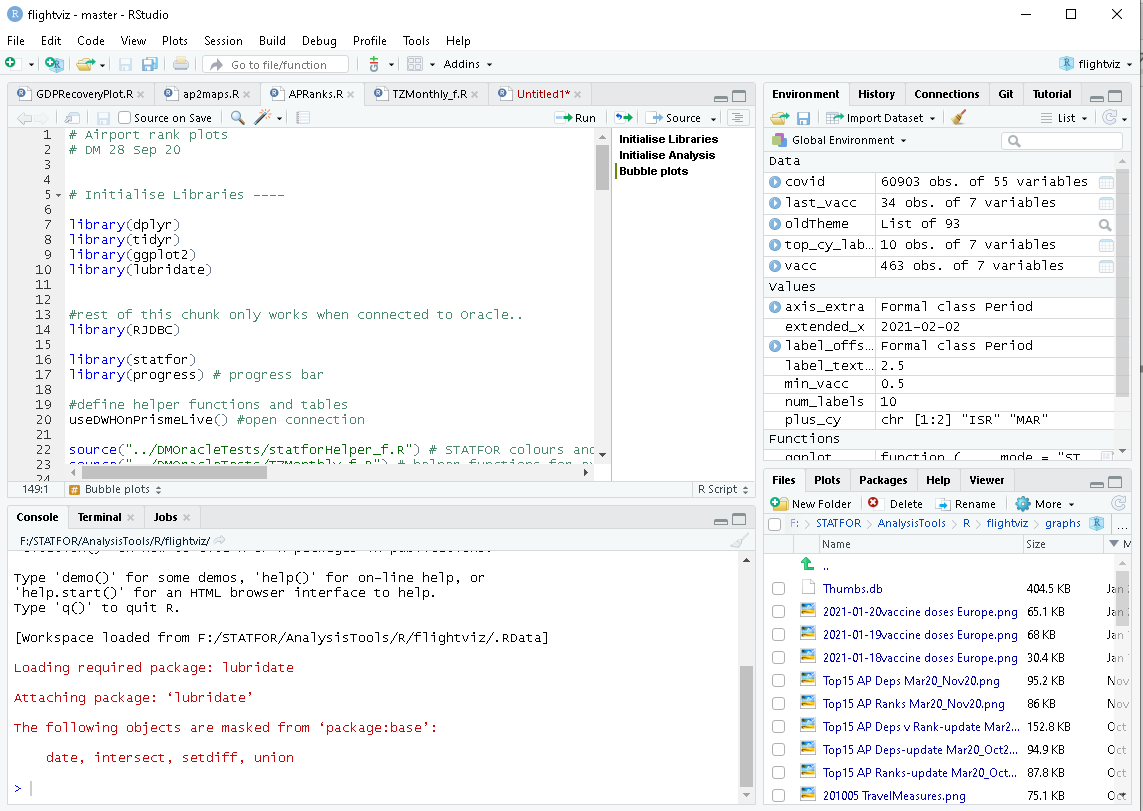
\includegraphics[width=0.75\textwidth,height=\textheight]{images/RStudio.png}
\caption{RStudio snapshot}
\end{figure}

The main panes of the screen are:

\begin{itemize}
\tightlist
\item
  Top left: source code, shown as a number of tabs one for each file;
\item
  Bottom left: the `console', which is a scratchpad for entering code, and where log output is usually shown (and some other tabs which we don't need here);
\item
  Top right: the `environment' and `history' tabs are of main interest. Environment is where you can explore all the data you've created. History is useful for re-doing something, particularly as you can search for code.
\item
  Bottom right: This has several important tabs

  \begin{itemize}
  \tightlist
  \item
    Files: for exploring files within a project, can be quicker than using the windows explorer
  \item
    Plots: is where plots will appear (usually)
  \item
    Packages: is for checking which packages are installed, or active (see TBD)
  \item
    Help: all the details of the functions that you will need - this is usually quicker to use than googling a function (though the help files come up when you google, from various providers).
  \end{itemize}
\end{itemize}

The buttons that appear around the panes are context-sensitive: they will change according to the type of file that you have open.

There are some hot-keys for moving rapidly around the panes: I most use ctrl-1 to go to the source code, ctrl-2 for the console. You can then guess the others.

Recent versions of \texttt{RStudio} have a tutorial (tab in top right pane) if you need more detail.

\hypertarget{first-project}{%
\section{First project}\label{first-project}}

While you can work with `bare' files of R code, we think it's tidier to use `projects', for two main reasons: you can keep several shorter files of code together, which makes it easier to navigate; and a project automatically remembers which directory it's working in, so you can manage data input and output and graphic output more neatly.

Create yourself a new project `File/New Project', selecting the options new project (not new package), give it the name `justlearning' and browse to put it in your personal R directory. (TBD templates).

It will open without a code panel, because you have no code yet. It looks like this.
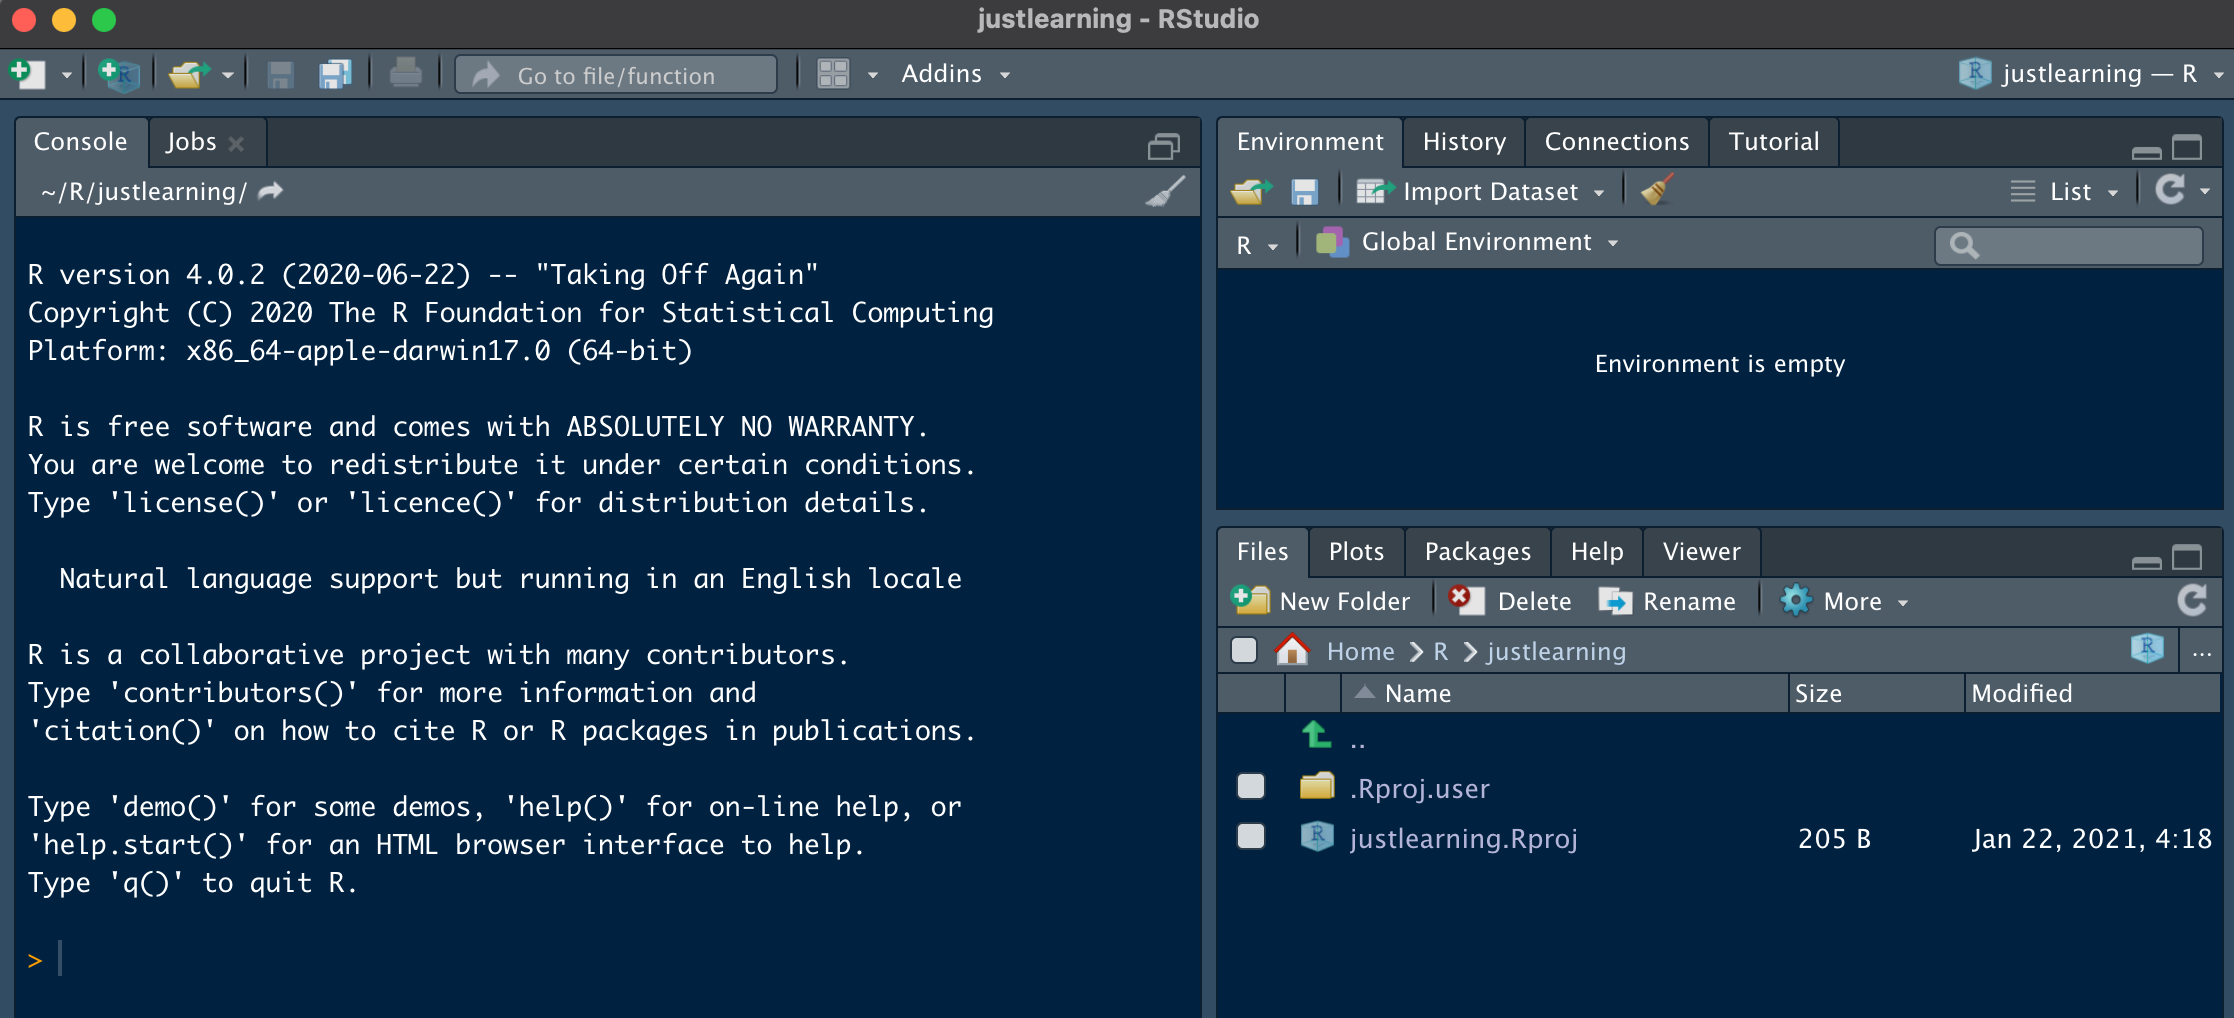
\includegraphics[width=0.75\textwidth,height=\textheight]{images/NewJustLearning.png}

You can already execute R code in the console (bottom left, ctrl-2), but we want to save and organise code. So we do a bit more organising, and then in the next section, create a file for the code.

In this book we'll assume that projects always keep data in the \texttt{data} directory, and save graphs to the \texttt{graphs} directory. You can create these quickly in your new project by copying the code (quick-copy icon appears top right in the code block) and pasting it into the console (and press return).

\begin{Shaded}
\begin{Highlighting}[]
\CommentTok{\# good to have these in every project}
\FunctionTok{dir.create}\NormalTok{(}\StringTok{"data"}\NormalTok{)}
\FunctionTok{dir.create}\NormalTok{(}\StringTok{"graphs"}\NormalTok{)}
\end{Highlighting}
\end{Shaded}

If for some reason the directories already exist, don't worry, you'll just get a warning. You can also do this manually using `New Folder' in the files tab (ctrl-5), but then look out for lower case! You could even use your operating system file explorer - these are just ordinary directories (`folders').

When you quit RStudio it will save any data and open files in your project. So you can re-open and continue from where you left off. If you've opened very large files, just beware that saving a copy as you close can take some time. (see TBD)

\hypertarget{first-code}{%
\section{First code}\label{first-code}}

Now you've got a blank project, add a new blank R script using \texttt{File/New\ File/R\ Script}, or the `file plus' icon top left. It appears in the source code pane, top left.

Immediately save it; `chapter2' for example. The name isn't critical here, but avoid spaces and punctuation. By default, it will be saved to the top level in the project. This is fine for many projects, though in some cases we might choose to organise code differently.

Type this code into your script, either manually or copy paste.

\begin{Shaded}
\begin{Highlighting}[]
\DecValTok{3} \SpecialCharTok{+} \DecValTok{4}
\CommentTok{\# I know pi}
\NormalTok{pi}
\DecValTok{1}\SpecialCharTok{:}\DecValTok{50}
\FunctionTok{cos}\NormalTok{(pi}\SpecialCharTok{/}\DecValTok{3}\NormalTok{) }\CommentTok{\# angle is in radians}
\end{Highlighting}
\end{Shaded}

Unlike in the console, it doesn't get executed as you type. You have to run it. Usually you're either:

\begin{itemize}
\tightlist
\item
  stepping through code, running a bit at a time, in which case ctrl-enter (cmd-enter on the Mac) is easy to use: it runs where the cursor currently sits, and then moves to the next line of code, jumping over comments that are preceded by \texttt{\#};
\item
  running all the code, which you can do by pressing the `source' button (or select all and ctrl-enter).
\end{itemize}

Output appears in the console as a running log.

\hypertarget{packages}{%
\section{First packages}\label{packages}}

A `package' provides a collection of functions, often some data and sometimes some new data types. If you're starting in R, and just aiming to find your way around in and use code, then mostly what you need to know is how to load packages (and what that means), and a little about the more common ones. That's what we cover in this section sections.

\hypertarget{package-basics}{%
\subsection{Package basics}\label{package-basics}}

Some packages come bundled with a basic installation of `R', such as \texttt{base} which provides, as the name suggests, many of the most basic functions. But there are thousands of other packages, coming from:

\begin{itemize}
\tightlist
\item
  \href{https://cran.r-project.org}{CRAN} or various `mirror' (official copy) sites hosted elsewhere, such as at Ghent University. These packages have been through a degree of quality control, and are preferred to the less official sources.
\item
  \href{https://github.com}{Github} and other public repositories. We share some there, such as \href{https://github.com/david6marsh/codaTaxi}{CODA taxi times} and the \href{https://github.com/euctrl-pru/portal}{PRC dashboard}.
\item
  Home-made. Making them is out of the scope of the book, but you will want to load the \texttt{statfor} package (TBD) created by Sebastien Thonnard that builds some access to Eurocontrol datawarehouses as well as nice formatting.
\end{itemize}

There are two\footnote{actually, there's a third, but that's too much detail for here} steps to using a package, and sometimes these get confused:

\begin{enumerate}
\def\labelenumi{\arabic{enumi})}
\tightlist
\item
  Installation. You type \texttt{install.packages("dplyr")} and R finds the files for that package and saves them on your machine or on a network drive. So the files are available. You've done the shopping and the food is in the kitchen cupboards.
\item
  Attaching or Loading. You have to make a package \emph{available} for use for your session. You've pulled the ingredients for your recipe out of the cupboard and they're on the kitchen table. If there's a difference between `attaching' and `loading' then it doesn't matter here.
\end{enumerate}

A very few packages are automatically loaded at the start of the session. In the packages pane, a package is listed if it is installed and ticked if it's loaded. In the screenshot, just the \texttt{base} package is loaded of the ones listed.

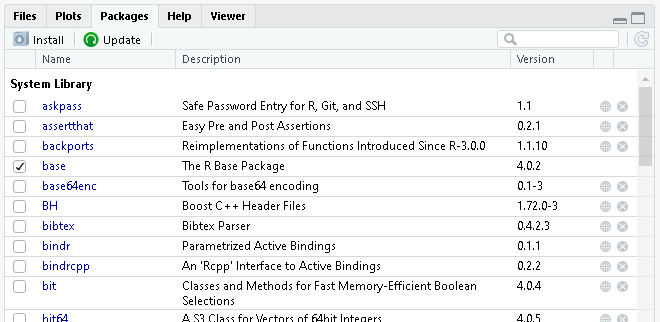
\includegraphics[width=0.75\textwidth,height=\textheight]{images/packages.png}

Clicking on the package name takes you to the documentation. There's a manual for all functions together, as a pdf, but it's usually easier to use the help pane to get the same material, and perhaps copy examples from the end of each help entry. More importantly here there are links to \textbf{vignettes}, and often now to websites with more info. Vignettes are not little stickers, but essential how-to guides mixing text and code; often this can provide a skeleton that you can copy and adapt to your own need.

You can load a package by ticking the box, but normally it's done in code, as in this example.

\begin{Shaded}
\begin{Highlighting}[]
\FunctionTok{library}\NormalTok{(lubridate) }\CommentTok{\# lots of date{-}related functions.}
\end{Highlighting}
\end{Shaded}

Two packages can define a function with the same name. That is not something CRAN controls, and when there's a clash, on loading the second one `masks' the first, as in the message displayed above. Sometimes, as an alternative to loading the full package, you might see in code a `two colon' usage, such as \texttt{base::union}. This is very common inside packages (it's recommended), and it's a way to insist that the first package version of the function should be used.

There are often many different functions that you could use to achieve the same result, eg \texttt{base::paste()} and \texttt{stringr::str\_c()} both concatenate strings (tbd). There's an art in R to doing the most with the minimum number of packages, since it takes time to find your way around the functions in a package. That's like the satisfaction of making the recipe from things you already have in the cupboard.

But sometimes, you just don't want to make the flaky pastry yourself. There are times when you're looking at a complex task and should be thinking `surely someone has already tackled this in R?'. A little googling might find you most of the pieces already in place.

In a way, you develop a personal `dialect' of R, from the packages you choose to use most often. We'll discuss one of the most common dialects, the \texttt{tidyverse}, in more detail in the next section.

\hypertarget{tidyverse}{%
\subsection{Tidyverse}\label{tidyverse}}

The \href{https://www.tidyverse.org}{tidyverse} is our chosen dialect, in the sense that in most cases we'll use the functions and data structures, and way of organising, that go with this collection of packages. There's a lot of excellent documentation already available, so we will explain some basics here, and introduce other elements as we need them for flight data examples.

The \emph{tidy} in `tidyverse' refers to a \href{https://r4ds.had.co.nz/tidy-data.html}{tidy data structure}: a table with each variable in its own column and each observation on one row. While we often put years across the table, and countries down the side, this is not `tidy'.

\begin{table}

\caption{\label{tab:twotables}An untidy table.}
\centering
\begin{tabular}[t]{lrr}
\toprule
Country & Flights2019 & Flights2020\\
\midrule
France & 1.3 & 1.5\\
Germany & 5.2 & 6.0\\
\bottomrule
\end{tabular}
\end{table}

\begin{table}

\caption{\label{tab:twotables}An tidy table.}
\centering
\begin{tabular}[t]{lrr}
\toprule
Country & Year & Flights\\
\midrule
France & 2019 & 1.3\\
Germany & 2020 & 5.2\\
France & 2019 & 1.5\\
Germany & 2020 & 6.0\\
\bottomrule
\end{tabular}
\end{table}

The main data structure used by the tidyverse is the dataframe, although increasingly the tidyverse prefers the `tibble' \texttt{tbl}, which is a specific sort of dataframe. (TBD) We won't worry about the differences here.

For most `quick pieces of code', the easiest is to start with a \texttt{library(tidyverse)} to load all the parts of the tidyverse. If you were writing a package, that wouldn't be very efficient, because there's quite a lot of it. Sometimes you'll see individual parts of the tidyverse loaded including:

\begin{itemize}
\tightlist
\item
  \texttt{ggplot2}: lots of plotting functions (see TBD)
\item
  \texttt{dplyr}: for manipulating and processing data
\item
  \texttt{tidyr}: for tidying data, such as pivot-table like actions, or splitting columns.
\end{itemize}

And there are packages which are on the outskirts of the `tidyverse' which get announced when you load.

\begin{Shaded}
\begin{Highlighting}[]
\FunctionTok{library}\NormalTok{(tidyverse)}
\end{Highlighting}
\end{Shaded}

These include \texttt{lubridate} and \texttt{stringr} which we've already mentioned.

\hypertarget{filetypes}{%
\section{File types}\label{filetypes}}

You will see lots of different file types (ie file extensions). The main ones to remember are:

\begin{itemize}
\tightlist
\item
  \texttt{.R}, \texttt{.Rmd}: both contain R code, though \texttt{.Rmd} is actually `r markdown' which is a mix of code and text;
\item
  \texttt{.RProj}: contains an R `project' - if you see one of these in the directory, this is the one to open - everything else works from there (see TBD);
\item
  \texttt{.rda}, \texttt{.RDS}: are different types of data file. R works easily also with \texttt{.csv} and \texttt{.xls(x)} see TBD.
\end{itemize}

\hypertarget{whats-gone-wrong-1}{%
\section{What's gone wrong?}\label{whats-gone-wrong-1}}

If you see a window like this, then you have started R rather than RStudio. That is a GUI and you can use it to execute R code, but you'll find RStudio easier for all but the quickest snippets of code. 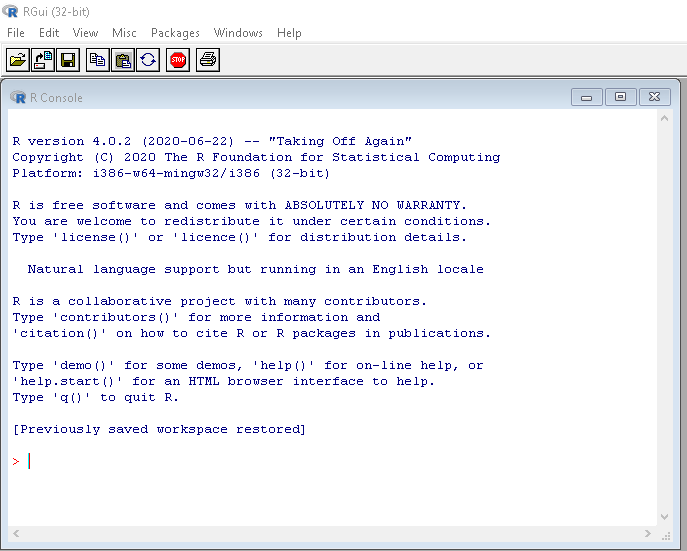
\includegraphics[width=0.5\textwidth,height=\textheight]{images/RGui.png}

If it keeps on happening you will find it helpful to associate R files (\texttt{.R,\ .RMD} and others) with RStudio rather than R.

If you get errors saying a certain package is only compatible with version xx and higher (of R), and you think you've recently updated, are you sure you updated R rather than RStudio? The RStudio version is found from the top menu `RStudio/About R Studio', the R version is seen when you first start up (see the image just above), or is printed if you type \texttt{version} in the console (see TBD).

If you're searching in `help' and a function isn't appearing, for example in the drop-down as you type, it is probably because it comes from a package that isn't loaded. You can finish typing, and the system will search and may find it, but also some other less good matches. Or if you know the package name, you can type \texttt{?ggplot2::geom\_line} for example, in the console to go straight there.

\hypertarget{test-yourself}{%
\section{Test yourself}\label{test-yourself}}

\hypertarget{questions}{%
\subsection{Questions}\label{questions}}

\begin{enumerate}
\def\labelenumi{\arabic{enumi}.}
\tightlist
\item
  In which pane will you (usually) find the help on functions?
\item
  Which of these provides a graphical user interface (GUI): R, RStudio?
\item
  Which ctrl-key combination takes you to the environment pane?
\item
  What does an \texttt{.rda} file contain?
\item
  What's the difference between typing into a source file and into the console?
\item
  What is a `vignette'?
  7 (teaser) What does \texttt{3\ +\ 1:3} give?
\end{enumerate}

\hypertarget{answers}{%
\subsection{Answers}\label{answers}}

\begin{enumerate}
\def\labelenumi{\arabic{enumi}.}
\tightlist
\item
  Bottom right.
\item
  Both, though you'll nearly always want to use RStudio.
\item
  CTRL-8
\item
  R data
\item
  With the console, code is executed as each line is completed.
\item
  An extended entry in the documentation showing how to put the functions of the packages together.
\item
  \texttt{4\ 5\ 6}
\end{enumerate}

\hypertarget{first-look-at-data-and-co2-emissions}{%
\chapter{\texorpdfstring{First look at data and CO\textsubscript{2} Emissions}{First look at data and CO2 Emissions}}\label{first-look-at-data-and-co2-emissions}}

It's hard to get far in an analysis without first looking at the data to ask questions such as:

\begin{itemize}
\tightlist
\item
  What variables are there? Do I know what they all mean?
\item
  What time period does it cover?
\item
  Which countries, or airports etc, are included?
\end{itemize}

In this chapter, we introduce some of the ways to take a quick look at your data. We introduce some data on CO\textsubscript{2} emissions per European State from aviation.

\begin{tabular}{l}
\hline
In this chapter\\
\hline
`read\_xlsx()`, `<-`, `summary`, `str`, environment pane, `View()`, `unique`, `head`, `c()`, `[]`, `ggplot()`\\
\hline
\end{tabular}

Re-open your \texttt{justlearning} project and start a new source file, to copy and paste the examples into. This starts a new R session, which means you have to re-load the package(s) that you need.

\begin{Shaded}
\begin{Highlighting}[]
\FunctionTok{suppressPackageStartupMessages}\NormalTok{(}\FunctionTok{library}\NormalTok{(tidyverse)) }\CommentTok{\# without lots of messages filling up the book}
\end{Highlighting}
\end{Shaded}

\hypertarget{loadco2}{%
\section{\texorpdfstring{Looking at data: CO\textsubscript{2} Data}{Looking at data: CO2 Data}}\label{loadco2}}

We use public data on national CO\textsubscript{2} emissions from aviation available on the \href{https://ansperformance.eu/data/}{EUROCONTROL/AIU website}. We choose this, apart from the interest in the data themselves, because it's a small set so quick to download, and it's already tidy (each variable in one column).

\begin{Shaded}
\begin{Highlighting}[]
\CommentTok{\# download the file to the data folder}
\CommentTok{\# download.file("https://ansperformance.eu/download/xls/CO2\_emissions\_by\_state.xlsx", }
\CommentTok{\#               "data/CO2\_emissions\_by\_state.xlsx")}

\CommentTok{\# load from the DATA worksheet {-} case sensitive!}
\NormalTok{aviation\_co2 }\OtherTok{\textless{}{-}}\NormalTok{ readxl}\SpecialCharTok{::}\FunctionTok{read\_xlsx}\NormalTok{(}\StringTok{"data/CO2\_emissions\_by\_state.xlsx"}\NormalTok{, }
                                  \AttributeTok{sheet =} \StringTok{"DATA"}\NormalTok{)}
\end{Highlighting}
\end{Shaded}

We've already seen the \texttt{function(parameter)} way to call a function in the \texttt{cos(pi/3)} example. Now we have \texttt{something\ \textless{}-\ function(parameter,\ parameter)}. This is a peculiarity of R that you just need to get used to. Think of it as saying: create \texttt{something} in the environment (without saying what it is just yet); then fill it (\texttt{\textless{}-}) with; the results of the \texttt{function}.

Now that the Excel is downloaded, comment out the 2 lines, because we don't need to keep downloading if you happen to re-run the code. If there were frequent updates, maybe you would keep downloading. See (TBD) for an example. See the Excel, now in your project \texttt{data} folder, for disclaimer and details.

International conventions mean that CO\textsubscript{2} emissions are measured from flights departing airports in a State. \texttt{read\_xlsx} automatically selects the first row as variable names.

\begin{Shaded}
\begin{Highlighting}[]
\FunctionTok{summary}\NormalTok{(aviation\_co2)}
\end{Highlighting}
\end{Shaded}

\begin{verbatim}
##       YEAR       STATE_NAME         STATE_CODE        Y_CO2_QTY_TONNES        Y_TF        
##  Min.   :2010   Length:432         Length:432         Min.   :       1   Min.   :      2  
##  1st Qu.:2012   Class :character   Class :character   1st Qu.:  196430   1st Qu.:  16603  
##  Median :2015   Mode  :character   Mode  :character   Median : 1042641   Median :  56292  
##  Mean   :2015                                         Mean   : 4223363   Mean   : 205720  
##  3rd Qu.:2017                                         3rd Qu.: 3308375   3rd Qu.: 225938  
##  Max.   :2019                                         Max.   :37260380   Max.   :1265392
\end{verbatim}

The \texttt{summary} function is fairly basic, but it gives a quick feel for what's in the data. Often more helpful with numeric than character, but also useful for spotting if there are missing values \texttt{NA}, of which there are none here.

In this dataset we have:

\begin{itemize}
\tightlist
\item
  YEAR: An integer, not a date, but read\_xlsx reads this as a real number.
\item
  STATE\_NAME, STATE\_CODE: A long name and the 2-letter `country code' derived from the ICAO 4-letter communication address, of which the less said, the better.
\item
  Y\_CO2\_QTY\_TONNES: Total annual CO2 emissions, in (metric) tonnes.
\item
  Y\_TF: Total flights. Presumably this is departing flights (TBD)
\end{itemize}

There are three other important ways to explore the data. Firstly in the environment pane (top right, CTRL-8), where you can click the blue arrow-disk to see a summary. You get much the same thing in the console by typing \texttt{str(aviation\_co2)} where \texttt{str} is for `structure'. You should see something like this.

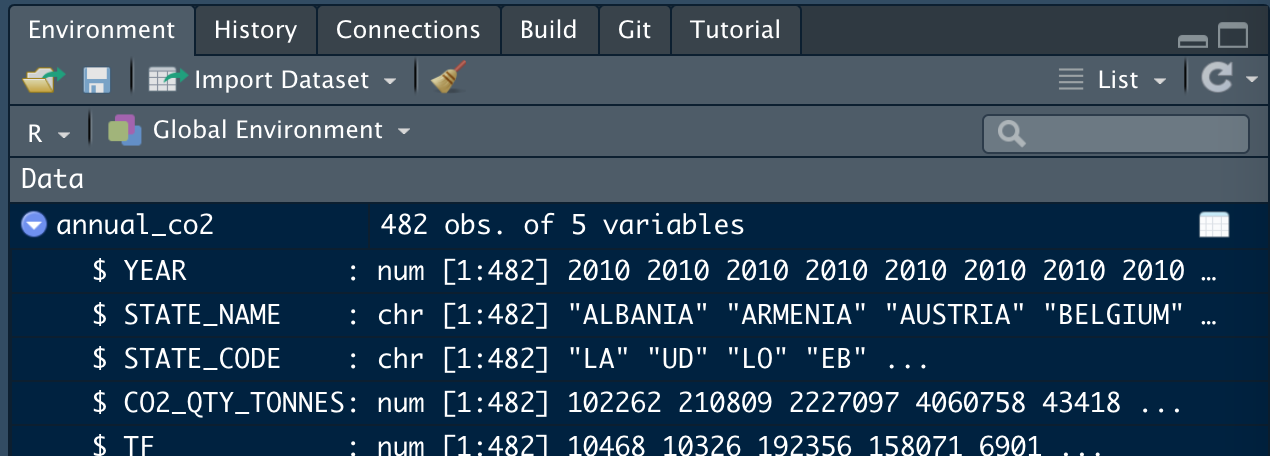
\includegraphics{images/CO2inEnvironment.png}

We can see that there are 3 numeric variables (\texttt{num}) and 3 character variables (\texttt{chr}). All 5 variables have the same number of observations (432 - but maybe this is more by the time you download it). In a tibble or data.frame the columns are always the same length.

The second way, because this is a tibble, is just to type its name in the console. {[}Try it{]} This is useful but just bear in mind that for some data structures, this might fill up your console with a lot of output. Save it for when you're sure you've a tibble. You can check by typing \texttt{class(my\_thing)} into the console to see if \texttt{my\_thing} is a tibble (shown as \texttt{tbl}).

The third way gives a way to explore every observation. Click on the dataset name next to the blue arrow or type \texttt{View(aviation\_co2)} in the console (sorry about the upper case `V') and you get a tabular data explorer, which allows you to sort and filter. You should see something like this. Try out the sorting and filtering in the view window.

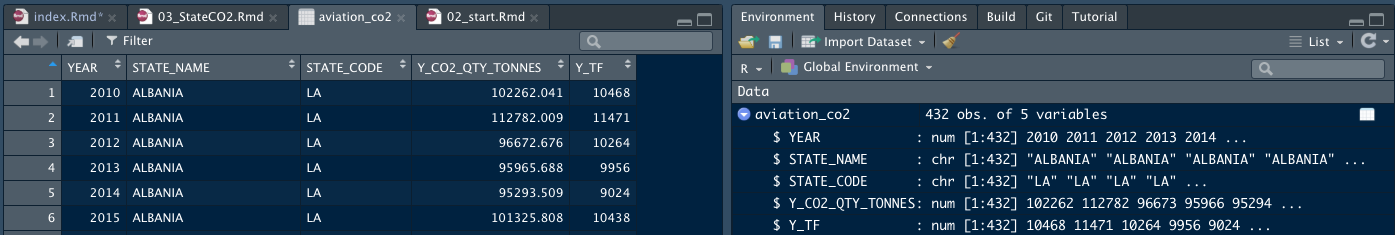
\includegraphics{images/CO2inViewAndEnvironment.png}

\hypertarget{extracting-variables}{%
\section{Extracting variables}\label{extracting-variables}}

To answer more questions about the data there are some more tools to summarise the values that it takes. We saw \texttt{summary()} works for numeric values, but what about discrete ones?

There are several ways to pull one variable out of your data. We'll use the \texttt{\$} notation, partly because there's a reminder of this in the environment tab.

\begin{Shaded}
\begin{Highlighting}[]
\CommentTok{\# pull out all values in the column}
\NormalTok{state\_vbl }\OtherTok{\textless{}{-}}\NormalTok{ aviation\_co2}\SpecialCharTok{$}\NormalTok{STATE\_NAME}

\NormalTok{states }\OtherTok{\textless{}{-}} \FunctionTok{unique}\NormalTok{(state\_vbl)}
\end{Highlighting}
\end{Shaded}

Look in the environment pane, \texttt{state\_vbl} is listed under `Values'. It's a (column) vector, one of the simple data types in R which is why it's listed under `Values' and not under `Data'. You've just pulled a column out of \texttt{aviation\_co2} so not surprising that it has the same number of rows as \texttt{aviation\_co2}. And the first values are all ALBANIA, or were when this book was compiled.

Really we want to know how many different States there are, and which ones. \texttt{unique} does what it says, and we've saved these as \texttt{states}; a variable name which to me implies `unique States'. You can tell how many there are from the environment pane, or you could use \texttt{length(states)}. {[}How many are there?{]}

To inspect all of these values you can just type \texttt{states} into the console, a good way to check the spelling of some, perhaps. {[}Try this.{]}

The order in which the elements are shown is as in the original data, there's no careless re-ordering. If you've worked with SAS PROC SQL or other languages, it might come as a relief to hear that, in R, the order of rows stays where it's put until you say otherwise; none of this sorting before every operation. We'll see some ways to handle `top' values later (TBD - top\_n)

So in this case, even if the \texttt{states} are in alphabetical order, that's just because the original Excel file was.

\hypertarget{extracting-a-few-values}{%
\section{Extracting a few values}\label{extracting-a-few-values}}

We've just seen how to pull a variable out of a tibble. How do we extract one or more values out of the vector that we created?

The \texttt{states} are quite a lot to show in the console. If you had even more you might just want to see a few. The code chunk above shows that \texttt{head()} is useful for showing you the first ones (6 by default).

\begin{Shaded}
\begin{Highlighting}[]
\FunctionTok{head}\NormalTok{(states)}
\end{Highlighting}
\end{Shaded}

\begin{verbatim}
## [1] "ALBANIA"                "ARMENIA"                "AUSTRIA"               
## [4] "BELGIUM"                "BOSNIA AND HERZEGOVINA" "BULGARIA"
\end{verbatim}

If you want to pull out a single value, or a few of them, again there are multiple ways to do this, but the simplest is this. We show here two ways to select with a vector of numbers: creating a consecutive sequence of numbers (\texttt{1:3}); and creating a vector with an arbitrary selection (\texttt{c(1,\ 5,\ 10)}).

\begin{Shaded}
\begin{Highlighting}[]
\NormalTok{states[}\DecValTok{1}\NormalTok{]}
\end{Highlighting}
\end{Shaded}

\begin{verbatim}
## [1] "ALBANIA"
\end{verbatim}

\begin{Shaded}
\begin{Highlighting}[]
\NormalTok{states[}\DecValTok{3}\NormalTok{]}
\end{Highlighting}
\end{Shaded}

\begin{verbatim}
## [1] "AUSTRIA"
\end{verbatim}

\begin{Shaded}
\begin{Highlighting}[]
\NormalTok{states[}\DecValTok{1}\SpecialCharTok{:}\DecValTok{3}\NormalTok{]}
\end{Highlighting}
\end{Shaded}

\begin{verbatim}
## [1] "ALBANIA" "ARMENIA" "AUSTRIA"
\end{verbatim}

\begin{Shaded}
\begin{Highlighting}[]
\NormalTok{states[}\FunctionTok{c}\NormalTok{(}\DecValTok{1}\NormalTok{, }\DecValTok{5}\NormalTok{, }\DecValTok{10}\NormalTok{)]}
\end{Highlighting}
\end{Shaded}

\begin{verbatim}
## [1] "ALBANIA"                "BOSNIA AND HERZEGOVINA" "CZECHIA"
\end{verbatim}

We'll deal with subsetting the whole dataset, rather than just a vector, in the next chapter.

\hypertarget{co2-scatter-plot}{%
\section{\texorpdfstring{CO\textsubscript{2} Scatter plot}{CO2 Scatter plot}}\label{co2-scatter-plot}}

It's hard to beat a graph as a way to explore data. So we end the chapter exploring a simple graph.

The tidyverse way of doing this is to use \texttt{ggplot}.

\hypertarget{first-draft}{%
\subsection{First draft}\label{first-draft}}

In the most basic scatter plot we have the following components, joined with a \texttt{+}. This \texttt{+} is peculiar to \texttt{ggplot}; another lovable quirk of R. Learn it, but get used to the idea that you'll forget and use other conjunctions by mistake at times.

In the simplest code we have:

\begin{itemize}
\tightlist
\item
  \texttt{ggplot}: with parameters the data to use, and an `aesthetic' \texttt{aes};
\item
  \texttt{aes}: gives the x and y first, and here also says choose colour based on year;
\item
  \texttt{geom\_point}: says to plot points with these data, ie a scatter plot.
\end{itemize}

\begin{Shaded}
\begin{Highlighting}[]
\FunctionTok{ggplot}\NormalTok{(aviation\_co2, }
       \FunctionTok{aes}\NormalTok{(Y\_TF, Y\_CO2\_QTY\_TONNES, }\AttributeTok{colour =}\NormalTok{ YEAR)) }\SpecialCharTok{+}
  \FunctionTok{geom\_point}\NormalTok{() }
\end{Highlighting}
\end{Shaded}

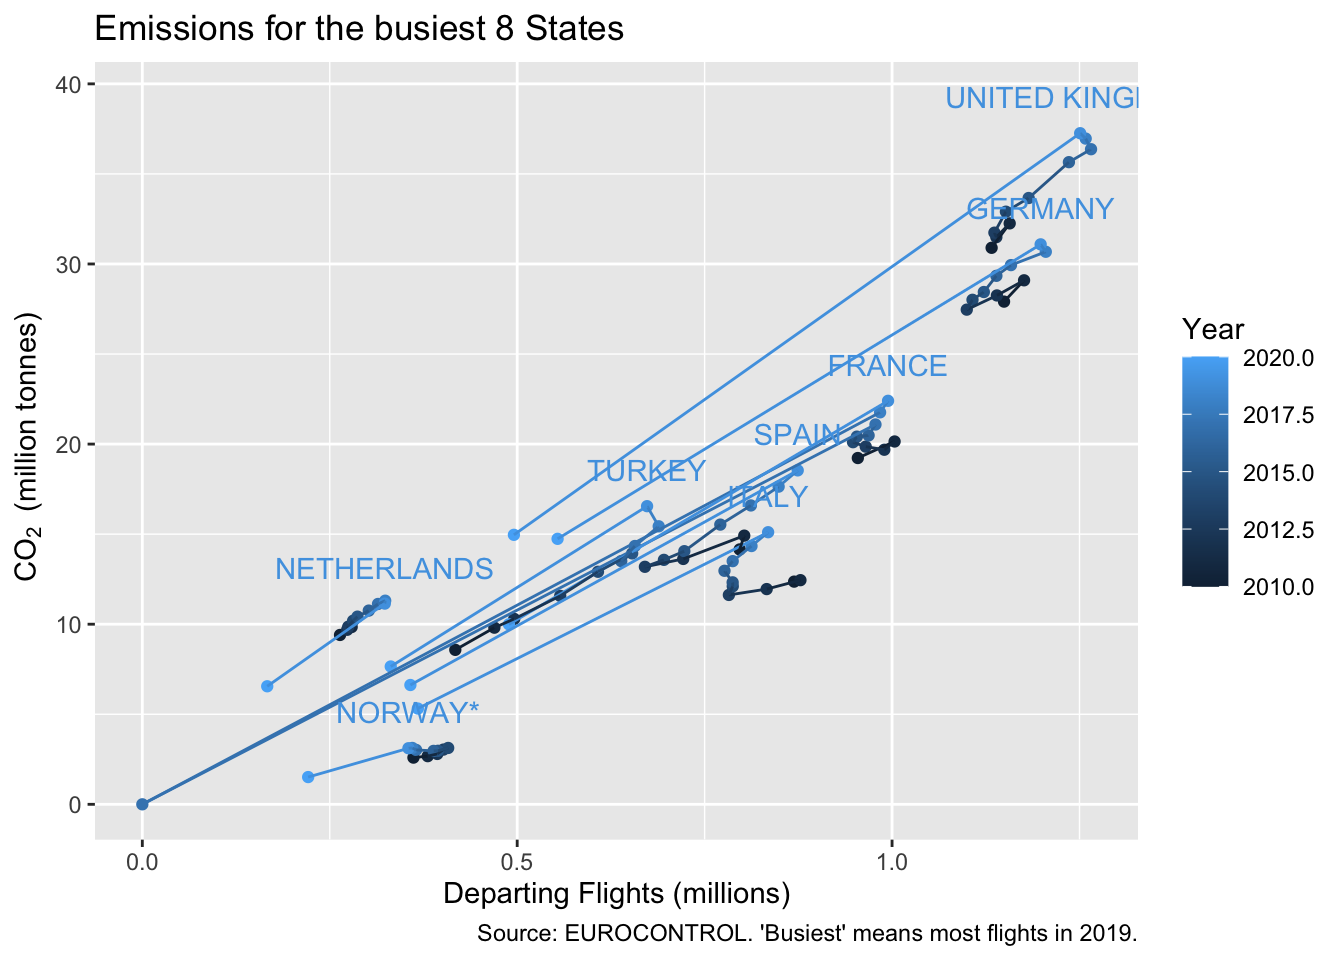
\includegraphics{flights_in_R_files/figure-latex/unnamed-chunk-5-1.pdf}

Even this simple example illustrates that:

\begin{itemize}
\tightlist
\item
  a parameter can be another function call \texttt{aes()};
\item
  we can specify parameters by order of appearance (\texttt{x} and \texttt{y} are first and second for \texttt{aes}) or by name (\texttt{colour}), or both;
\item
  \texttt{geom\_point} takes its aesthetics by default from the \texttt{ggplot} statement.
\end{itemize}

There's a (very) rough correlation along a diagonal line, but it would be interesting to know which States are above the line (more CO\textsubscript{2} per flight) and which below. And is the change gradual, or is there much variability?

\hypertarget{improve-the-titles}{%
\subsection{Improve the titles}\label{improve-the-titles}}

Let's at least label the axes so that someone else can see quickly what has been plotted. We can transform variables on the fly (using the rule that a parameter can be a function call, here to the function \texttt{/}), so let's convert both axes to millions.

The label on the legend is meaningful, but to avoid the block capitals we can change that too within the \texttt{labs} statement.

\begin{Shaded}
\begin{Highlighting}[]
\FunctionTok{ggplot}\NormalTok{(aviation\_co2, }\FunctionTok{aes}\NormalTok{(Y\_TF}\SpecialCharTok{/}\FloatTok{1e6}\NormalTok{, Y\_CO2\_QTY\_TONNES}\SpecialCharTok{/}\FloatTok{1e6}\NormalTok{, }\AttributeTok{colour =}\NormalTok{ YEAR)) }\SpecialCharTok{+}
  \FunctionTok{geom\_point}\NormalTok{() }\SpecialCharTok{+} 
  \FunctionTok{labs}\NormalTok{(}\AttributeTok{x =} \StringTok{"Departing Flights (millions)"}\NormalTok{, }
       \AttributeTok{y =} \StringTok{"CO2 (million tonnes)"}\NormalTok{,}
       \AttributeTok{colour =} \StringTok{"Year"}\NormalTok{,}
       \AttributeTok{title =} \StringTok{"Emissions per State"}\NormalTok{)}
\end{Highlighting}
\end{Shaded}

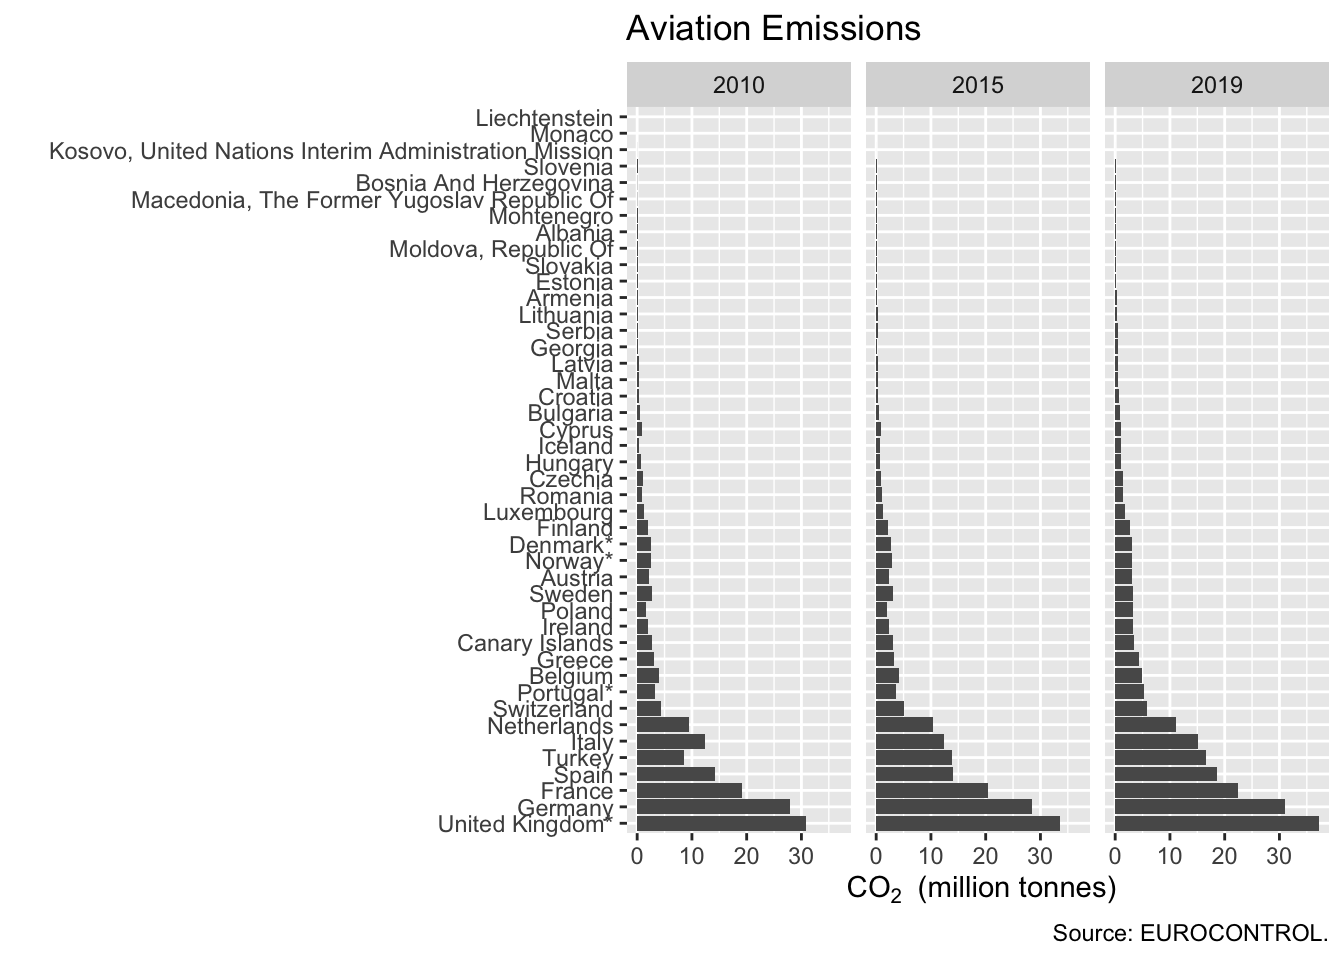
\includegraphics{flights_in_R_files/figure-latex/unnamed-chunk-6-1.pdf}

\hypertarget{statecluster}{%
\subsection{and with clustering by State}\label{statecluster}}

It's tempting to read the graph as having a number of small clusters, each with flights and CO\textsubscript{2} increasing with time, and assume that each of these corresponds to a single State. It would be nice to use the graph to see if that's true.

There are too many countries to give each its own shape (we'll see shapes used more effectively in TBD), but we can easily add a line to join the points for each State. {[}How do you think you would add a line?{]}

We need both to add a line, which follows the pattern of \texttt{geom\_point}, and group by State. That's done in the same way that we coloured by year, in the aesthetics. But there are several ways to plot a line \texttt{geom\_line} joins the points in x-axis order, we want data order, so that's \texttt{geom\_path}.

Out of a sense of neatness, we also add a subscript to CO\textsubscript{2}. The code \texttt{bquote(\textasciitilde{}CO{[}2{]}\textasciitilde{}"\ (million\ tonnes)")} took some googling and is cryptic, but it works!

\begin{Shaded}
\begin{Highlighting}[]
\FunctionTok{ggplot}\NormalTok{(aviation\_co2, }\FunctionTok{aes}\NormalTok{(Y\_TF}\SpecialCharTok{/}\FloatTok{1e6}\NormalTok{, Y\_CO2\_QTY\_TONNES}\SpecialCharTok{/}\FloatTok{1e6}\NormalTok{, }
                         \AttributeTok{colour =}\NormalTok{ YEAR, }\AttributeTok{group =}\NormalTok{ STATE\_NAME)) }\SpecialCharTok{+}
  \FunctionTok{geom\_point}\NormalTok{() }\SpecialCharTok{+} 
  \FunctionTok{geom\_path}\NormalTok{() }\SpecialCharTok{+}
  \FunctionTok{labs}\NormalTok{(}\AttributeTok{x =} \StringTok{"Departing Flights (millions)"}\NormalTok{, }
       \AttributeTok{y =} \FunctionTok{bquote}\NormalTok{(}\SpecialCharTok{\textasciitilde{}}\NormalTok{CO[}\DecValTok{2}\NormalTok{]}\SpecialCharTok{\textasciitilde{}}\StringTok{" (million tonnes)"}\NormalTok{),}
       \AttributeTok{colour =} \StringTok{"Year"}\NormalTok{,}
       \AttributeTok{title =} \StringTok{"Emissions per State"}\NormalTok{)}
\end{Highlighting}
\end{Shaded}

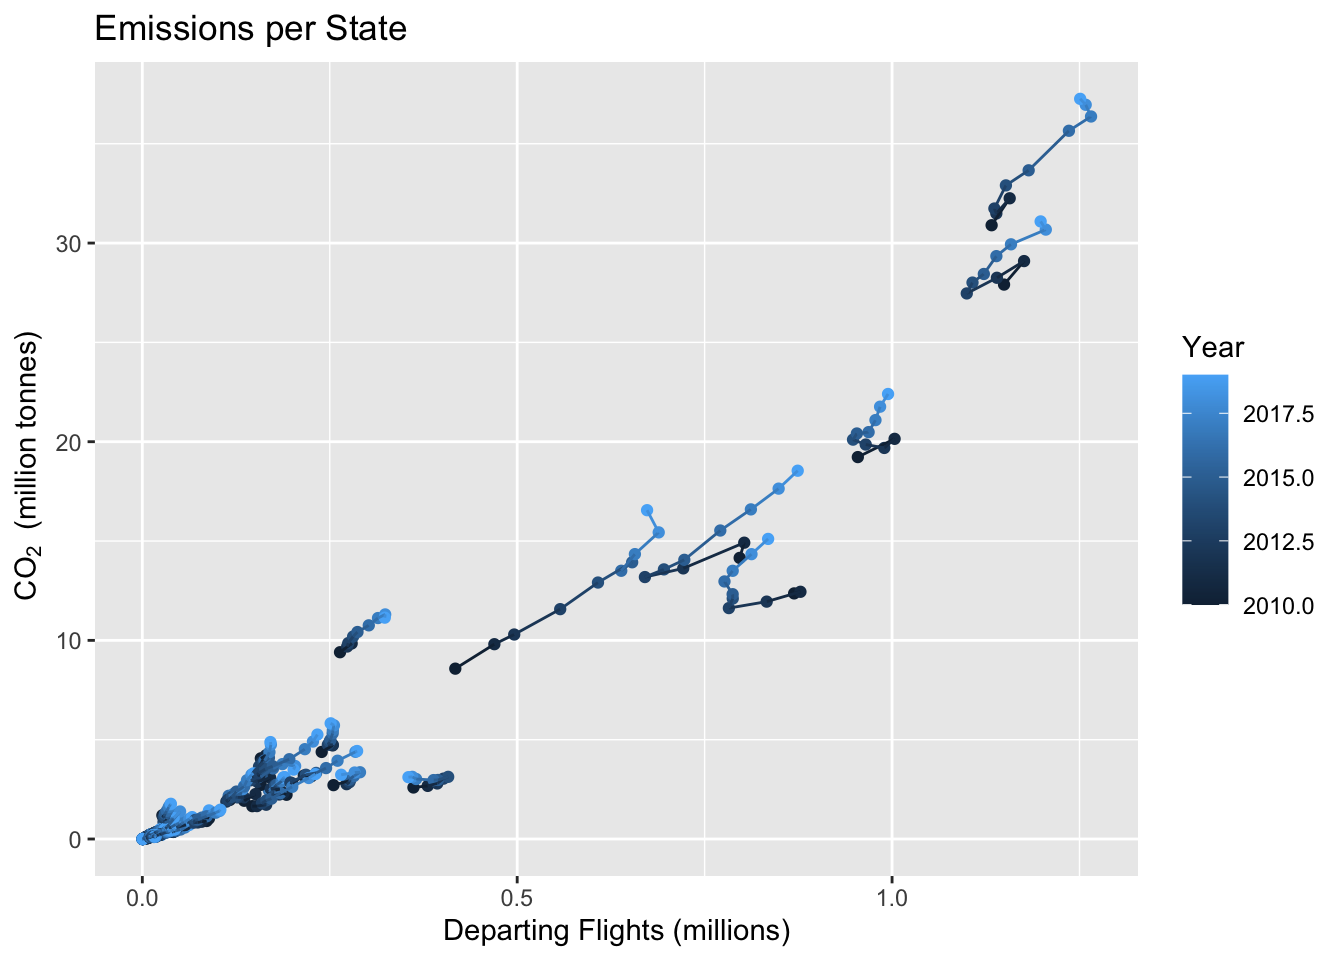
\includegraphics{flights_in_R_files/figure-latex/unnamed-chunk-7-1.pdf}

The graph isn't ready for a presentation yet, but a story is already emerging. The lines do the job of grouping the years for each State together. We see a graph with 6 busy States, 3 of which are fairly linear, so a relatively fixed CO\textsubscript{2}/flight. Three others are more variable from year to year.

Then there are two States, with flights in the 0.25-0.5 million flights range and that diverge from the main trend line. The remaining States rather overlap in this graph.

We'll find out how to pick out and label States in the next chapter.

\hypertarget{whats-gone-wrong-2}{%
\section{What's gone wrong?}\label{whats-gone-wrong-2}}

\hypertarget{test-yourself-1}{%
\section{Test yourself}\label{test-yourself-1}}

\hypertarget{questions-1}{%
\subsection{Questions}\label{questions-1}}

\begin{enumerate}
\def\labelenumi{\arabic{enumi})}
\tightlist
\item
  Use \texttt{head} to view the first 10 states.
\item
  Using the help file for \texttt{head}, how would you display the last 6 states?
\item
  Which State names are followed by '*'?
\item
  Print the distinct state ISO codes to the console.
\item
  Print the 3rd, 23rd and 33rd state names to the console.
\item
  What does \texttt{\textless{}-} do?
\item
  In \texttt{ggplot} what does \texttt{+} do?
\end{enumerate}

\hypertarget{answers-1}{%
\subsection{Answers}\label{answers-1}}

\begin{enumerate}
\def\labelenumi{\arabic{enumi})}
\tightlist
\item
  \texttt{head(states,\ 10)}
\item
  \texttt{head} is documented alongside \texttt{tail}: use \texttt{tail(states)}
\item
  (In my version of the data), typing \texttt{states} into the console, and by eye I see 4 States with a '*'. We'll see other ways to do this, later.
\item
  \texttt{unique(aviation\_co2\$STATE\_CODE)}
\item
  \texttt{states{[}c(3,\ 23,\ 33){]}}
\item
  It puts the results of whatever is on the right-hand side into the object on the left.
\item
  It connects parts of the definition of a graph together.
\end{enumerate}

\hypertarget{filtering-a-dataset-and-refining-the-co2-graph}{%
\chapter{\texorpdfstring{Filtering a dataset and refining the CO\textsubscript{2} graph}{Filtering a dataset and refining the CO2 graph}}\label{filtering-a-dataset-and-refining-the-co2-graph}}

In this chapter we improve the CO\textsubscript{2} emissions graph, \emph{en route} learning how to filter observations from a dataset, to add new variables, and to use the \texttt{pipe} operator \texttt{\%\textgreater{}\%}.

\begin{tabular}{l}
\hline
In this chapter\\
\hline
`filter()`, `==`, `\%in\%`, `mutate()`, `slice\_max()`, `\%>\%`, `geom\_text\_repel()`\\
\hline
\end{tabular}

On restarting your \texttt{justlearning} project, you should still have the \texttt{aviation\_co2} dataset in your environment, since RStudio saves these data and reloads on restart. If not, use the code in section @ref\{loadco2\} to load the Excel file from the \texttt{data} folder.

If you have closed RStudio and re-opened it, then you have a new session and need to reload packages, in this case \texttt{library(tidyverse)}.

\hypertarget{sequences-of-functions}{%
\section{Sequences of functions}\label{sequences-of-functions}}

It's time for a bit more syntax. We saw already that you can combine functions by making one the parameter to another. Or to put it another way, wrapping one around the other. As you combine more functions, this soon becomes hard to read, and you have to rely on the editor to help you spot whether you've enough brackets closed at the right point.

For that reason we use a different syntax, the `pipe' operator \texttt{\%\textgreater{}\%} introduced by the \texttt{magrittr} package and adopted by the tidyverse. If you learn only one control-key combination learn shift-ctrl-M (also shift-command-M on Mac). This must be the fastest way to type `\%\textgreater\%'! {[}Try it in your console.{]}

With a new line after each \texttt{\%\textgreater{}\%} and appropriate indenting (RStudio helps with that), you get code that looks like this. This says, fill \texttt{a} with what you get from dataset \texttt{b} after applying function \texttt{fun1}, then function \texttt{fun2}.

\begin{Shaded}
\begin{Highlighting}[]
\CommentTok{\# which is clearer}
\CommentTok{\# with a pipe?}
\NormalTok{a }\OtherTok{\textless{}{-}}\NormalTok{ b }\SpecialCharTok{\%\textgreater{}\%} 
  \FunctionTok{fun1}\NormalTok{(p1) }\SpecialCharTok{\%\textgreater{}\%} 
  \FunctionTok{fun2}\NormalTok{(p2, p3)}
\CommentTok{\# or without?}
\NormalTok{a }\OtherTok{\textless{}{-}} \FunctionTok{fun2}\NormalTok{(}\FunctionTok{fun1}\NormalTok{(b, p1), p2, p3)}
\end{Highlighting}
\end{Shaded}

The pipe syntax works because \texttt{fun1} actually has a parameter list that \emph{starts} with the dataset to which it should be applied \texttt{fun1(data,\ p1,...)}. So \texttt{b\ \%\textgreater{}\%\ fun1(p1)} is just another way of writing \texttt{fun1(b,\ p1)}. Or, the other way around, you can use \texttt{\%\textgreater{}\%} whenever you have a function whose first parameter is the dataset to be operated on. It turns out that this is true for very many of them, and the tidyverse is designed that way.

\hypertarget{filtering-datasets-and-logical-tests}{%
\section{Filtering datasets and Logical Tests}\label{filtering-datasets-and-logical-tests}}

As is so often the case, in R there are several of ways to select rows from a dataframe or tibble. We'll focus on the \texttt{filter(data,\ test)} function. For this we need to know how to construct a logical test.

There are three parts to this: the logic, the test functions and what's being tested. Logic is mostly given by \texttt{\&}, \texttt{!} and \texttt{\textbar{}}\footnote{that's a vertical bar, not an `l' or `I'} for `and', `not' and `or', grouped with round brackets in the normal way. The test functions are \emph{almost} as you might expect: \texttt{\textgreater{}}, \texttt{\textless{}}. However, in R you need to use \texttt{==} not \texttt{=} to test for equality. I suspect this creates the most common typo in R code! Check the documentation of \texttt{dplyr::filter} for a more complete list of test functions: in particular look out for \texttt{\%in\%}, which we will use shortly.

One really nice touch in \texttt{filter()} is in the third part: what's being tested. One of the trickiest bits of learning R is knowing how, within a function, to refer to one or more variables of the dataset. In \texttt{filter()} you can just use the name of the variable; so no quotes needed around the name, and the code assumes it is a variable from the \texttt{data} parameter, so no need to use \texttt{aviation\_co2\$}.

In this example, we don't push the result into a dataset (no \texttt{a\ \textless{}-}), so it gets printed out directly.

\begin{Shaded}
\begin{Highlighting}[]
\NormalTok{aviation\_co2 }\SpecialCharTok{\%\textgreater{}\%} 
  \FunctionTok{filter}\NormalTok{(YEAR }\SpecialCharTok{==} \DecValTok{2018} \SpecialCharTok{\&}\NormalTok{ STATE\_NAME }\SpecialCharTok{\%in\%} \FunctionTok{c}\NormalTok{(}\StringTok{"CZECHIA"}\NormalTok{, }\StringTok{"ALBANIA"}\NormalTok{))}
\end{Highlighting}
\end{Shaded}

\begin{verbatim}
## # A tibble: 2 x 5
##    YEAR STATE_NAME STATE_CODE Y_CO2_QTY_TONNES  Y_TF
##   <dbl> <chr>      <chr>                 <dbl> <dbl>
## 1  2018 ALBANIA    LA                  143871. 12744
## 2  2018 CZECHIA    LK                 1381672. 90679
\end{verbatim}

Note that:

\begin{itemize}
\tightlist
\item
  the order of the rows is as in the original dataset, not at all influenced by the order of the naming of the States in the test
\item
  \texttt{YEAR} and \texttt{STATE\_NAME} are `bare' strings, and are shorthand for \texttt{aviation\_co2\$YEAR} etc
\item
  but ``CZECHIA'' is a value of a variable so needs to be a string in quotes
\item
  and the test is case-sensitive.
\end{itemize}

\hypertarget{selecting-the-busiest-states}{%
\section{Selecting the busiest States}\label{selecting-the-busiest-states}}

In the previous chapter we selected the first-named States with \texttt{head()}. Now we do something more useful: selecting the top States by flights, using \texttt{slice\_max()}. We need to define this a bit more clearly. `Top' could mean in a particular year, or over the whole period (where flights have decreased as well as increased). We choose to mean `top by flights in 2019'. This is partly out of habit (this is often the meaning) and partly because we need to introduce fewer new bits of R to implement it.

The code is like this. A final novelty is that we use \texttt{pull()} which, as its help-file says, does the same as \texttt{\$} (learned in the last chapter) but looks nicer in pipes.

\begin{Shaded}
\begin{Highlighting}[]
\NormalTok{top\_states }\OtherTok{\textless{}{-}}\NormalTok{ aviation\_co2 }\SpecialCharTok{\%\textgreater{}\%} 
  \FunctionTok{filter}\NormalTok{(YEAR }\SpecialCharTok{==} \DecValTok{2019}\NormalTok{) }\SpecialCharTok{\%\textgreater{}\%}     \CommentTok{\# top in year 2019}
  \FunctionTok{slice\_max}\NormalTok{(Y\_TF, }\AttributeTok{n =} \DecValTok{8}\NormalTok{) }\SpecialCharTok{\%\textgreater{}\%}  \CommentTok{\# top 8 }
  \FunctionTok{pull}\NormalTok{(STATE\_NAME) }
\end{Highlighting}
\end{Shaded}

\texttt{slice\_max()} is a good example of how R changes with time. New versions of packages introduce minor or major changes. Sometimes a function is \texttt{superseded} (left to rot), other times it may be \texttt{deprecated} (you have some time to switch to a new version before it's removed). The function \texttt{top\_n}, which you might see lying around in legacy code, has been superseded by \texttt{slice\_max()}. {[}Check out the documentation of \texttt{top\_n} for some of the reasons.{]}

These changes mean that just updating to the latest version of the package is not always the best idea, because you might have to spend some time checking for changes. It also means that, when searching on the web for hints, snippets and answers, you need to look at the date of the answer. \texttt{ggplot} in particular has changed quite a bit, so answers more than 5 years old or so might not be that helpful.

\hypertarget{co2-graph-for-the-top-states}{%
\section{\texorpdfstring{CO\textsubscript{2} graph for the top States}{CO2 graph for the top States}}\label{co2-graph-for-the-top-states}}

With \texttt{top\_states} in place we can easily plot the data for the busiest States.

We update the title, and add a footnote (\texttt{caption}) to explain what's going on. We could have created a new dataset, eg \texttt{top\_co2\ \textless{}-\ aviation\_co2\ \%\textgreater{}\%\ filter(STATE\_NAME\ \%in\%\ top\_states)}, and then used this in the \texttt{ggplot}. But we only plan to use this filter once, so to avoid cluttering the environment with datasets, we filter `on the fly', within the \texttt{ggplot} statement. In this case, this is a matter of personal preference. If the datasets were a lot larger, and we intended analysing and transforming just the top States in further graphs, the decision might be different.

\begin{Shaded}
\begin{Highlighting}[]
\FunctionTok{ggplot}\NormalTok{(aviation\_co2 }\SpecialCharTok{\%\textgreater{}\%} 
         \FunctionTok{filter}\NormalTok{(STATE\_NAME }\SpecialCharTok{\%in\%}\NormalTok{ top\_states), }
       \FunctionTok{aes}\NormalTok{(Y\_TF}\SpecialCharTok{/}\FloatTok{1e6}\NormalTok{, Y\_CO2\_QTY\_TONNES}\SpecialCharTok{/}\FloatTok{1e6}\NormalTok{, }
           \AttributeTok{colour =}\NormalTok{  STATE\_NAME)) }\SpecialCharTok{+}
  \FunctionTok{geom\_point}\NormalTok{() }\SpecialCharTok{+} 
  \FunctionTok{geom\_path}\NormalTok{() }\SpecialCharTok{+}
  \FunctionTok{labs}\NormalTok{(}\AttributeTok{x =} \StringTok{"Departing Flights (millions)"}\NormalTok{, }
       \AttributeTok{y =} \FunctionTok{bquote}\NormalTok{(}\SpecialCharTok{\textasciitilde{}}\NormalTok{CO[}\DecValTok{2}\NormalTok{]}\SpecialCharTok{\textasciitilde{}}\StringTok{" (million tonnes)"}\NormalTok{),}
       \AttributeTok{colour =} \StringTok{"Year"}\NormalTok{,}
       \AttributeTok{title =} \StringTok{"Emissions for the busiest 8 States"}\NormalTok{,}
       \AttributeTok{caption =} \StringTok{"Source: EUROCONTROL. \textquotesingle{}Busiest\textquotesingle{} means most flights in 2019."}\NormalTok{)}
\end{Highlighting}
\end{Shaded}

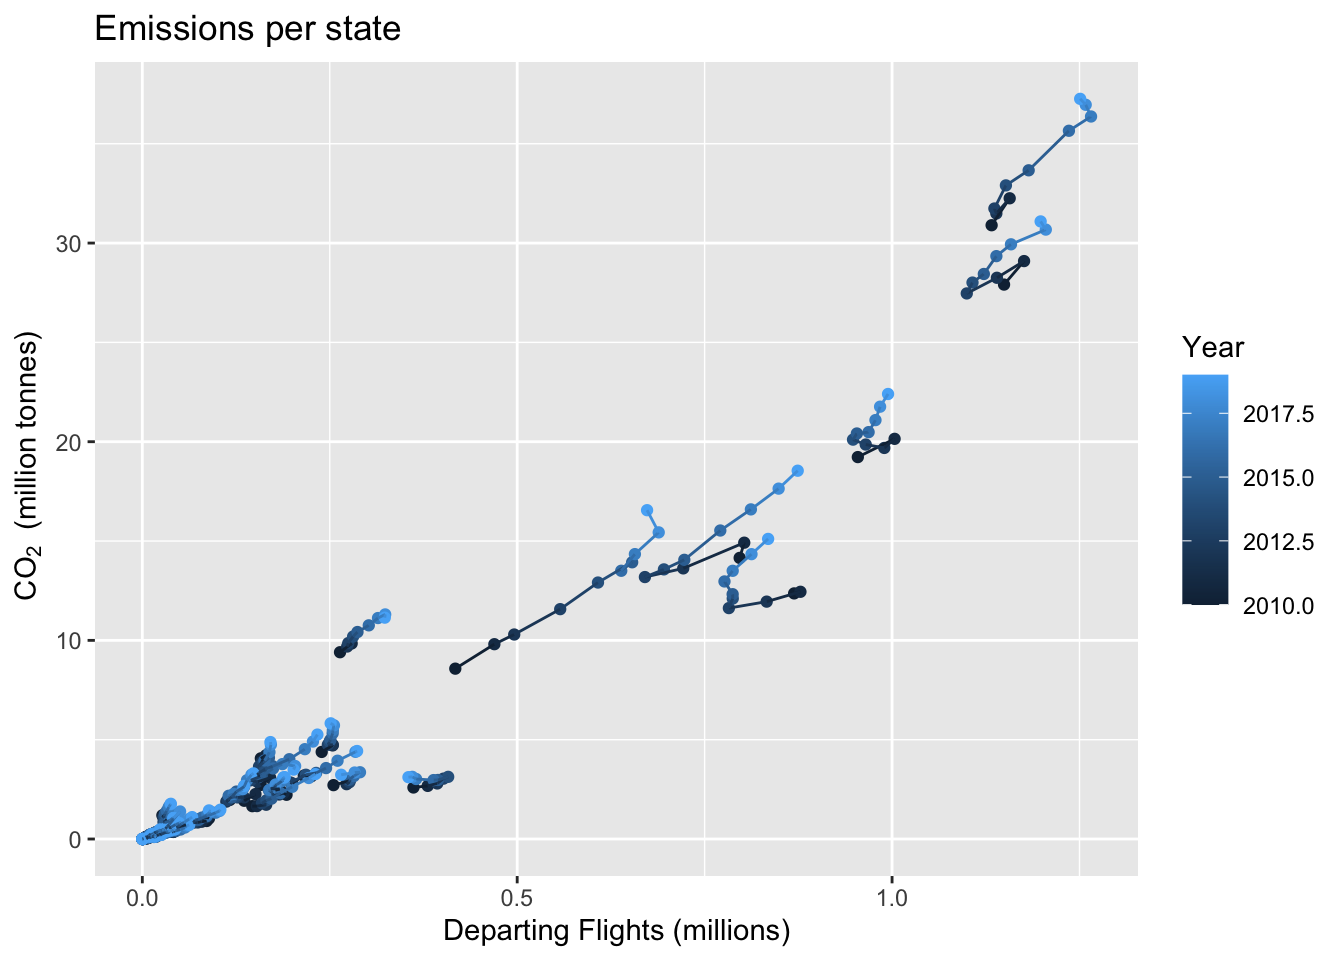
\includegraphics{flights_in_R_files/figure-latex/unnamed-chunk-11-1.pdf}

One advantage of filtering on the fly is that we can change on the fly. {[}Change the filter to the States \emph{not} in the top 8. It takes one key press. Re-run the graph. Update the titles too.{]}

As an analyst, I really want to know which country is which. With just 8 States shown, maybe I can use symbols? At one level it's quick to do. Just replace \texttt{group\ =} with \texttt{shape\ =}. {[}Try this.{]} \texttt{ggplot} complains that it doesn't really like using more than 6 symbols, because it becomes hard for the reader to jump between legend and graph. We could roll with it and learn how to extend the pallette, but is there another solution.

We can separate States by colours. Again, quite quick: replace \texttt{colour\ =\ YEAR,\ group\ =\ STATE\_NAME} with \texttt{colour\ =\ STATE\_NAME}. {[}Try this.{]} The line means we can work out the ordering of the years easily, so losing the year isn't a big issue here. But eight colours is also a lot to tell apart. Even without colour blindness, you might think they're clear but when projected onto a screen or printed or on a tiny phone screen, perhaps not.

\hypertarget{labelling-the-co2-graph}{%
\section{\texorpdfstring{Labelling the CO\textsubscript{2} graph}{Labelling the CO2 graph}}\label{labelling-the-co2-graph}}

It's relatively easy to follow a slightly different route: adding State names directly to the graph. This is done with \texttt{geom\_text} added to the \texttt{ggplot}. We only want to label the point in 2019 rather than all years, so we create a new variable which is empty except in rows for the year 2019. \texttt{mutate(a\ =\ ...)} is the function for adding a variable `a' to the dataset\footnote{and we use lower case for the variable name, because that's our preference, even if the imported names don't do this}. \texttt{if\_else()} is how we give a value for only some years. Notice that, like the \texttt{filter()}, we can refer to other variables in \texttt{aviation\_co2} without inverted commas.

This time, we amend the \texttt{aviation\_co2} dataset itself, because we want to be able to use this in several places, not just in a single graph. The syntax \texttt{a\ \textless{}-\ a\ \%\textgreater{}\%\ ...} follows the same pattern as you saw earlier, but you're overwriting the original dataset.

The \texttt{geom\_text()} \emph{inherits} all the aesthetics from the \texttt{ggplot} function, so it already knows where to find x and y coordinates, and what colour to use. We still need to tell \texttt{geom\_text()} where to find the labels. This is also an aesthetic.

\begin{Shaded}
\begin{Highlighting}[]
\NormalTok{aviation\_co2 }\OtherTok{\textless{}{-}}\NormalTok{ aviation\_co2 }\SpecialCharTok{\%\textgreater{}\%} 
  \FunctionTok{mutate}\NormalTok{(}\AttributeTok{state\_label =} \FunctionTok{if\_else}\NormalTok{(YEAR }\SpecialCharTok{==} \DecValTok{2019}\NormalTok{, STATE\_NAME, }\StringTok{""}\NormalTok{))}

\FunctionTok{ggplot}\NormalTok{(aviation\_co2 }\SpecialCharTok{\%\textgreater{}\%} 
         \FunctionTok{filter}\NormalTok{(STATE\_NAME }\SpecialCharTok{\%in\%}\NormalTok{ top\_states), }
       \FunctionTok{aes}\NormalTok{(Y\_TF}\SpecialCharTok{/}\FloatTok{1e6}\NormalTok{, Y\_CO2\_QTY\_TONNES}\SpecialCharTok{/}\FloatTok{1e6}\NormalTok{, }
           \AttributeTok{colour =}\NormalTok{ YEAR, }\AttributeTok{group =}\NormalTok{ STATE\_NAME)) }\SpecialCharTok{+}
  \FunctionTok{geom\_point}\NormalTok{() }\SpecialCharTok{+} 
  \FunctionTok{geom\_path}\NormalTok{() }\SpecialCharTok{+}
  \FunctionTok{geom\_text}\NormalTok{(}\FunctionTok{aes}\NormalTok{(}\AttributeTok{label =}\NormalTok{ state\_label)) }\SpecialCharTok{+}
  \FunctionTok{labs}\NormalTok{(}\AttributeTok{x =} \StringTok{"Departing Flights (millions)"}\NormalTok{, }
       \AttributeTok{y =} \FunctionTok{bquote}\NormalTok{(}\SpecialCharTok{\textasciitilde{}}\NormalTok{CO[}\DecValTok{2}\NormalTok{]}\SpecialCharTok{\textasciitilde{}}\StringTok{" (million tonnes)"}\NormalTok{),}
       \AttributeTok{colour =} \StringTok{"Year"}\NormalTok{,}
       \AttributeTok{title =} \StringTok{"Emissions for the busiest 8 States"}\NormalTok{,}
       \AttributeTok{caption =} \StringTok{"Source: EUROCONTROL. \textquotesingle{}Busiest\textquotesingle{} means most flights in 2019."}\NormalTok{)}
\end{Highlighting}
\end{Shaded}

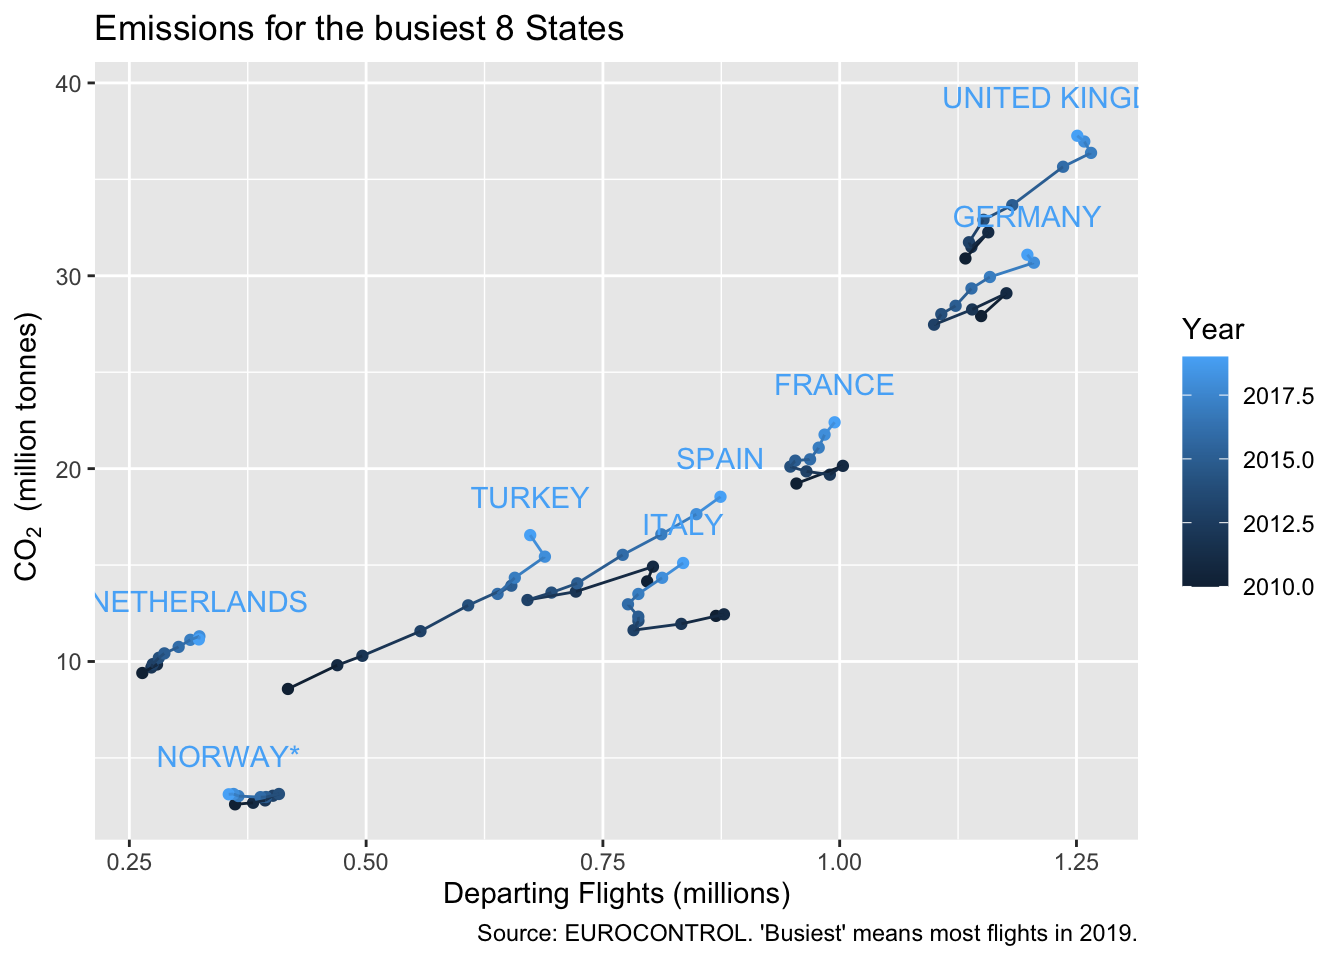
\includegraphics{flights_in_R_files/figure-latex/unnamed-chunk-12-1.pdf}

This is close, but not quite good enough. The text is centred on the point, and this creates some ugly overlaps. There are lots of options in \texttt{geom\_text()} to adjust the position, and you'll find lots of examples on the web {[}Check the documentation for a start.{]}. So we could spend time adjusting the positions. But this is a first example of the rule: `surely someone has already come across this problem?'. Someone has indeed spent time to come up with good ways to deconflict and position labels on graphs. The package is called \texttt{ggrepel}, which you might need to install with \texttt{install.packages("ggrepel")}, and it provides a `drop in' replacement for \texttt{geom\_text} naturally called \texttt{geom\_text\_repel}. To avoid using \texttt{library("ggrepel")} when we're just using one function, we use the double-colon syntax in the code.

The defaults for this function work pretty well in this particular case. But there are a couple of things I'd like to fix: the block capitals and the year legend. Title case would be nicer, so we convert the \texttt{STATE\_NAME} using the \texttt{stringr} package function \texttt{str\_to\_title()}. \texttt{stringr} is already loaded as part of the tidyverse, and since most of its functions begin `str\_' it's quite easy to start searching in the help pane for the right one {[}Try this.{]}. In this case \texttt{state\_label} already exists and we overwrite it.

The other thing to improve is the year scale, which shows with meaningless decimals. We use a quick-ish fix, rather than the tidiest-possible solution. (see TBD) Scales, whether the axes or colours, are controlled by \texttt{ggplot} functions starting \texttt{scales\_} in this case \texttt{scales\_colour\_steps()} gets us a scale that shows the individual years. This is a `dirty' solution in the sense that, if the data for 2020 get included, you might need to tweak the code; but then, we've hard-coded 2019 in a number of places, so this is dirty elsewhere. We'll see cleaner options later (TBD).

\begin{Shaded}
\begin{Highlighting}[]
\NormalTok{aviation\_co2 }\OtherTok{\textless{}{-}}\NormalTok{ aviation\_co2 }\SpecialCharTok{\%\textgreater{}\%} 
  \FunctionTok{mutate}\NormalTok{(}\AttributeTok{state\_label =} \FunctionTok{if\_else}\NormalTok{(YEAR }\SpecialCharTok{==} \DecValTok{2019}\NormalTok{, }\FunctionTok{str\_to\_title}\NormalTok{(STATE\_NAME), }\StringTok{""}\NormalTok{))}

\FunctionTok{ggplot}\NormalTok{(aviation\_co2 }\SpecialCharTok{\%\textgreater{}\%} 
         \FunctionTok{filter}\NormalTok{(STATE\_NAME }\SpecialCharTok{\%in\%}\NormalTok{ top\_states), }
       \FunctionTok{aes}\NormalTok{(Y\_TF}\SpecialCharTok{/}\FloatTok{1e6}\NormalTok{, Y\_CO2\_QTY\_TONNES}\SpecialCharTok{/}\FloatTok{1e6}\NormalTok{, }
           \AttributeTok{colour =}\NormalTok{ YEAR, }\AttributeTok{group =}\NormalTok{ STATE\_NAME)) }\SpecialCharTok{+}
  \FunctionTok{geom\_point}\NormalTok{() }\SpecialCharTok{+} 
  \FunctionTok{geom\_path}\NormalTok{() }\SpecialCharTok{+}
\NormalTok{  ggrepel}\SpecialCharTok{::}\FunctionTok{geom\_text\_repel}\NormalTok{(}\FunctionTok{aes}\NormalTok{(}\AttributeTok{label =}\NormalTok{ state\_label)) }\SpecialCharTok{+}
  \FunctionTok{scale\_colour\_steps}\NormalTok{(}\AttributeTok{n.breaks =} \DecValTok{8}\NormalTok{, }\AttributeTok{show.limits =} \ConstantTok{TRUE}\NormalTok{) }\SpecialCharTok{+}
  \FunctionTok{labs}\NormalTok{(}\AttributeTok{x =} \StringTok{"Departing Flights (millions)"}\NormalTok{, }
       \AttributeTok{y =} \FunctionTok{bquote}\NormalTok{(}\SpecialCharTok{\textasciitilde{}}\NormalTok{CO[}\DecValTok{2}\NormalTok{]}\SpecialCharTok{\textasciitilde{}}\StringTok{" (million tonnes)"}\NormalTok{),}
       \AttributeTok{colour =} \StringTok{"Year"}\NormalTok{,}
       \AttributeTok{title =} \StringTok{"Emissions for the busiest 8 States"}\NormalTok{,}
       \AttributeTok{caption =} \StringTok{"Source: EUROCONTROL. \textquotesingle{}Busiest\textquotesingle{} means most flights in 2019."}\NormalTok{)}
\end{Highlighting}
\end{Shaded}

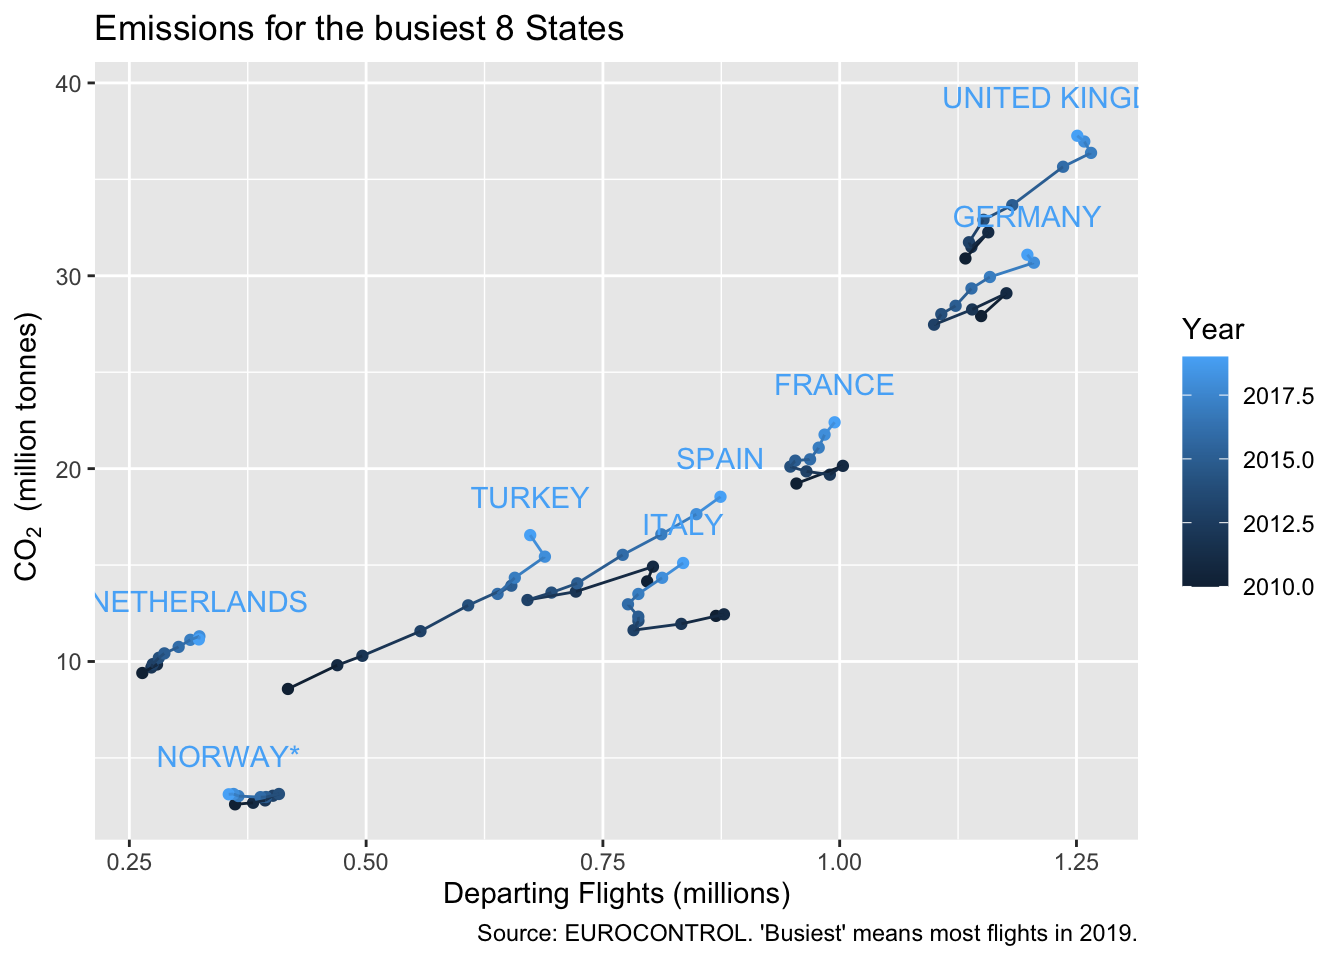
\includegraphics{flights_in_R_files/figure-latex/unnamed-chunk-13-1.pdf}

\hypertarget{what-does-the-graph-say-about-co2}{%
\section{\texorpdfstring{What does the graph say about CO\textsubscript{2}?}{What does the graph say about CO2?}}\label{what-does-the-graph-say-about-co2}}

Longer-haul flights use heavier aircraft and therefore the proportion of long-haul flights in your national mix is a major influence on CO\textsubscript{2} per flight. For example, the Netherlands has more CO\textsubscript{2} per flight than Norway: Norway has a significant domestic (so short-range) market, which the Netherlands does not. These have been relatively stable.

The UK also has a proportionally larger long-haul market. And a decline in its domestic market has led to quite a rapid increase in CO\textsubscript{2} per flight in recent years.

So, the graph helps to build a story: though we needed some supporting information to provide some of the explanation. It has also become clear that we're interested in CO\textsubscript{2} per flight. See the exercises for a graph on that more directly.

\hypertarget{whats-gone-wrong-3}{%
\section{What's gone wrong?}\label{whats-gone-wrong-3}}

It's inevitable that you will type \texttt{=} in tests where you mean \texttt{==}. Some functions have friendly messages, since this is so common. Others less so.

Watch that case! We are using the function \texttt{filter()}, not the function \texttt{Filter()} which is something else entirely.

\texttt{if\_else} is a fussy version of the base function \texttt{ifelse}, that we use here to maximise use of tidyverse functions. If it warns you that the `false' must be something, then it has your long-term interests at heart. It just means that it's a different type to the `true'. Compare \texttt{ifelse(1\textless{}2,"true",NA)} and \texttt{if\_else(1\textless{}2,"true",NA)} where \texttt{NA} is the code for missing.

It pays to looks closely at the graph and try to explain what you see. In fact, it was only once I'd tidied the colours up that I noticed that they were not in order along the line. I had used \texttt{geom\_line} (join in x-axis order) in place of \texttt{geom\_path} (join in data order). So story-telling can help debugging too. Also, it pays to read the help file, even if you think you know how the function works!

\hypertarget{exercises}{%
\section{Exercises}\label{exercises}}

\hypertarget{questions-2}{%
\subsection{Questions}\label{questions-2}}

\begin{itemize}
\tightlist
\item
  Adapt the graph to show the smallest 8 States instead. (Hints: What's the most likely counterpart to \texttt{slice\_max}? Closely-related functions are often to be found in the \emph{same} help file.)
\item
  Adapt the graph to show year on the x-axis and CO\textsubscript{2}/flight on the y-axis. (Hints: Mostly changing the first \texttt{aes()} and deleting some elements. For a pretty graph you might google how to hide the legend ``ggplot hide legend'', and how to set the breaks on the x-axis.)
\end{itemize}

\hypertarget{answers-2}{%
\subsection{Answers}\label{answers-2}}

\begin{itemize}
\tightlist
\item
  \texttt{geom\_text\_repel} uses call-out lines when it can't get the text close. You could experiment with making these a less confusing colour. You might also drop the `millions'.
\end{itemize}

\begin{Shaded}
\begin{Highlighting}[]
\NormalTok{small\_states }\OtherTok{\textless{}{-}}\NormalTok{ aviation\_co2 }\SpecialCharTok{\%\textgreater{}\%} 
  \FunctionTok{filter}\NormalTok{(YEAR }\SpecialCharTok{==} \DecValTok{2019}\NormalTok{) }\SpecialCharTok{\%\textgreater{}\%}     \CommentTok{\#  in year 2019}
  \FunctionTok{slice\_min}\NormalTok{(Y\_TF, }\AttributeTok{n =} \DecValTok{8}\NormalTok{) }\SpecialCharTok{\%\textgreater{}\%}  \CommentTok{\# smallest 8 }
  \FunctionTok{pull}\NormalTok{(STATE\_NAME)}

\FunctionTok{ggplot}\NormalTok{(aviation\_co2 }\SpecialCharTok{\%\textgreater{}\%} 
         \FunctionTok{filter}\NormalTok{(STATE\_NAME }\SpecialCharTok{\%in\%}\NormalTok{ small\_states), }
       \FunctionTok{aes}\NormalTok{(Y\_TF}\SpecialCharTok{/}\FloatTok{1e6}\NormalTok{, Y\_CO2\_QTY\_TONNES}\SpecialCharTok{/}\FloatTok{1e6}\NormalTok{, }
           \AttributeTok{colour =}\NormalTok{ YEAR, }\AttributeTok{group =}\NormalTok{ STATE\_NAME)) }\SpecialCharTok{+}
  \FunctionTok{geom\_point}\NormalTok{() }\SpecialCharTok{+} 
  \FunctionTok{geom\_path}\NormalTok{() }\SpecialCharTok{+}
\NormalTok{  ggrepel}\SpecialCharTok{::}\FunctionTok{geom\_text\_repel}\NormalTok{(}\FunctionTok{aes}\NormalTok{(}\AttributeTok{label =}\NormalTok{ state\_label)) }\SpecialCharTok{+}
  \FunctionTok{scale\_colour\_steps}\NormalTok{(}\AttributeTok{n.breaks =} \DecValTok{8}\NormalTok{, }\AttributeTok{show.limits =} \ConstantTok{TRUE}\NormalTok{) }\SpecialCharTok{+}
  \FunctionTok{labs}\NormalTok{(}\AttributeTok{x =} \StringTok{"Departing Flights (millions)"}\NormalTok{, }
       \AttributeTok{y =} \FunctionTok{bquote}\NormalTok{(}\SpecialCharTok{\textasciitilde{}}\NormalTok{CO[}\DecValTok{2}\NormalTok{]}\SpecialCharTok{\textasciitilde{}}\StringTok{" (million tonnes)"}\NormalTok{),}
       \AttributeTok{colour =} \StringTok{"Year"}\NormalTok{,}
       \AttributeTok{title =} \StringTok{"Emissions for the least{-}busy States"}\NormalTok{,}
       \AttributeTok{caption =} \StringTok{"Source: EUROCONTROL. \textquotesingle{}Busiest\textquotesingle{} means most flights in 2019."}\NormalTok{)}
\end{Highlighting}
\end{Shaded}

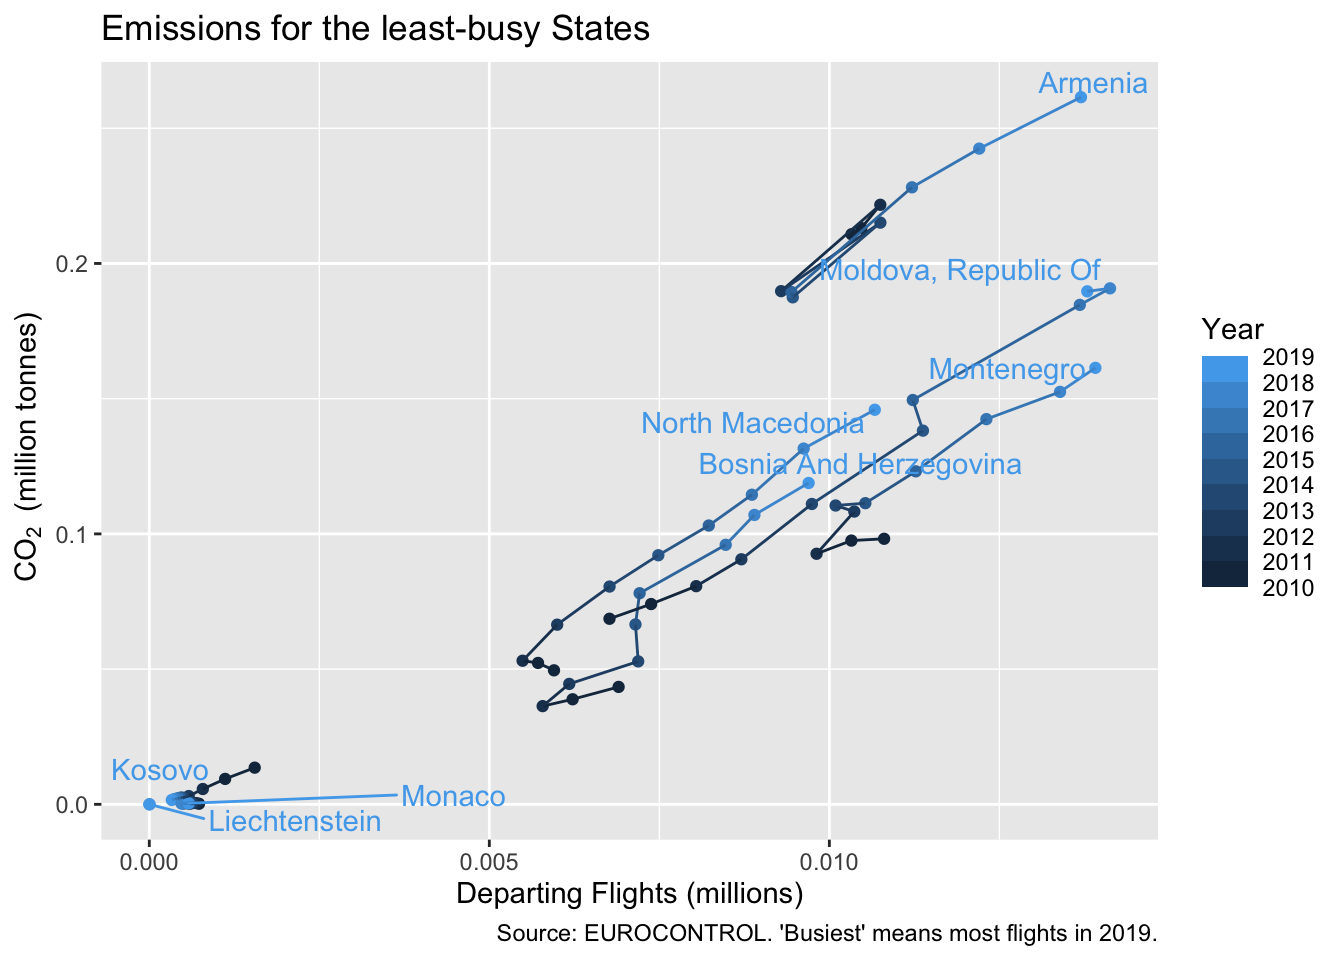
\includegraphics{flights_in_R_files/figure-latex/unnamed-chunk-14-1.pdf}

\begin{itemize}
\tightlist
\item
  A pedant might say this shouldn't be a line chart, but here's one possibility.
\end{itemize}

\begin{Shaded}
\begin{Highlighting}[]
\FunctionTok{ggplot}\NormalTok{(aviation\_co2 }\SpecialCharTok{\%\textgreater{}\%} 
         \FunctionTok{filter}\NormalTok{(STATE\_NAME }\SpecialCharTok{\%in\%}\NormalTok{ top\_states), }
       \FunctionTok{aes}\NormalTok{(YEAR, Y\_CO2\_QTY\_TONNES}\SpecialCharTok{/}\NormalTok{Y\_TF, }
           \AttributeTok{colour =}\NormalTok{ STATE\_NAME)) }\SpecialCharTok{+}
  \FunctionTok{geom\_path}\NormalTok{() }\SpecialCharTok{+} \CommentTok{\# I decided the points looked too heavy}
\NormalTok{  ggrepel}\SpecialCharTok{::}\FunctionTok{geom\_text\_repel}\NormalTok{(}\FunctionTok{aes}\NormalTok{(}\AttributeTok{label =}\NormalTok{ state\_label)) }\SpecialCharTok{+}
  \FunctionTok{theme}\NormalTok{(}\AttributeTok{legend.position =} \StringTok{"none"}\NormalTok{) }\SpecialCharTok{+}  \CommentTok{\# turn off legend}
  \FunctionTok{scale\_x\_continuous}\NormalTok{(}\AttributeTok{breaks =} \DecValTok{2010}\SpecialCharTok{:}\DecValTok{2019}\NormalTok{, }\AttributeTok{minor\_breaks =} \ConstantTok{NULL}\NormalTok{) }\SpecialCharTok{+} \CommentTok{\# control the breaks}
  \FunctionTok{labs}\NormalTok{(}\AttributeTok{x =} \StringTok{"Year"}\NormalTok{, }
       \AttributeTok{y =} \FunctionTok{bquote}\NormalTok{(}\SpecialCharTok{\textasciitilde{}}\NormalTok{CO[}\DecValTok{2}\NormalTok{]}\SpecialCharTok{\textasciitilde{}}\StringTok{" (tonnes per flight)"}\NormalTok{),}
       \AttributeTok{title =} \StringTok{"Emissions for the busiest 8 States"}\NormalTok{,}
       \AttributeTok{caption =} \StringTok{"Source: EUROCONTROL. \textquotesingle{}Busiest\textquotesingle{} means most flights in 2019."}\NormalTok{)}
\end{Highlighting}
\end{Shaded}

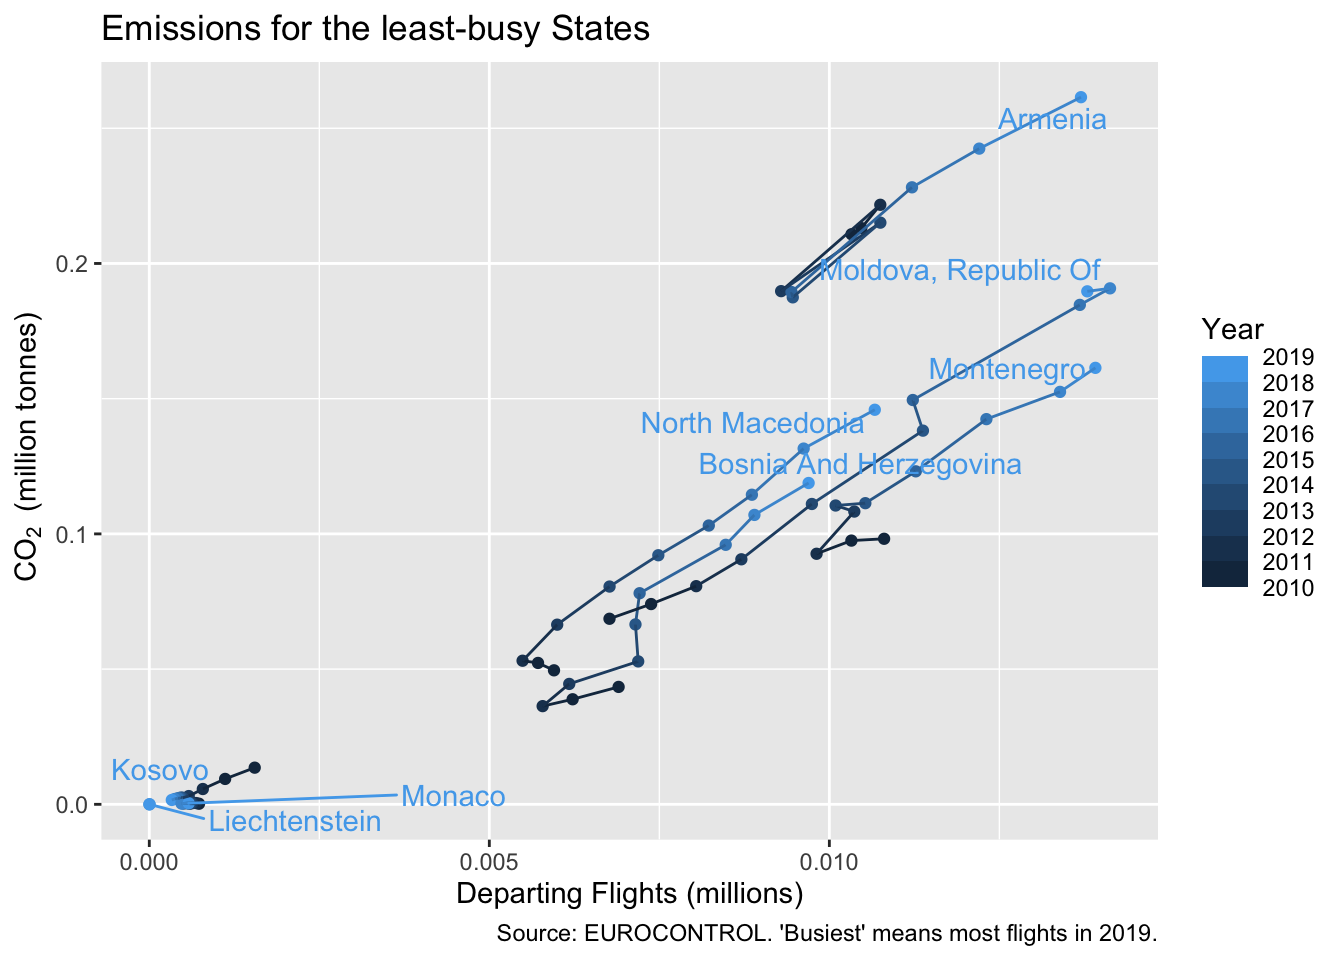
\includegraphics{flights_in_R_files/figure-latex/unnamed-chunk-15-1.pdf}

  \bibliography{book.bib,packages.bib}

\end{document}
